%\lstinputlisting[language=bash,basicstyle=\small]{python_codes/fieldstone_78/keywords.ascii}

\begin{center}
Code at \url{https://github.com/cedrict/fieldstone/tree/master/python_codes/fieldstone_78}
\end{center}

\par\noindent\rule{\textwidth}{0.4pt}

%%%%%%%%%%%%%%%%%%%%%%%%%%%%%%%%%%%%%%%%%%%%%%%%%%%%%%%%%%%%%%%%%%%%%%%%%%%%%%%%%%%%%%%%%%%%%%%%%%%%


Although the $Q_1\times P_0$ is not LBB-stable (see Section~\ref{MMM-ss:LBBcond})
it has been proven that some spatial arrangements of this element can be.
These are macro-elements, i.e. groupings of elements that are then repeated.
We will here consider:

\begin{itemize}
\item the regular macro-element (not really one, just a regular grid in practice).

\begin{center}
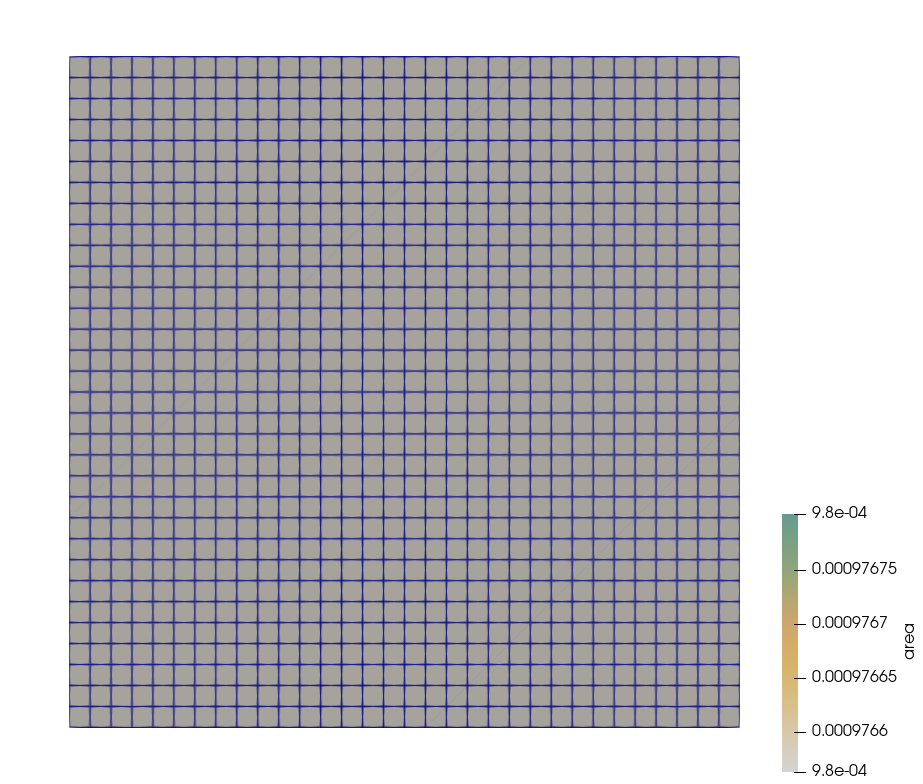
\includegraphics[width=5cm]{python_codes/fieldstone_78/images/16x16/area0.png}
\end{center}

\item the Stenberg (S) macro-element: it originates in \cite{sten84}.
It is also found in \cite{chba93}, \cite{brfo}, \cite{qizh07}.

\begin{center}
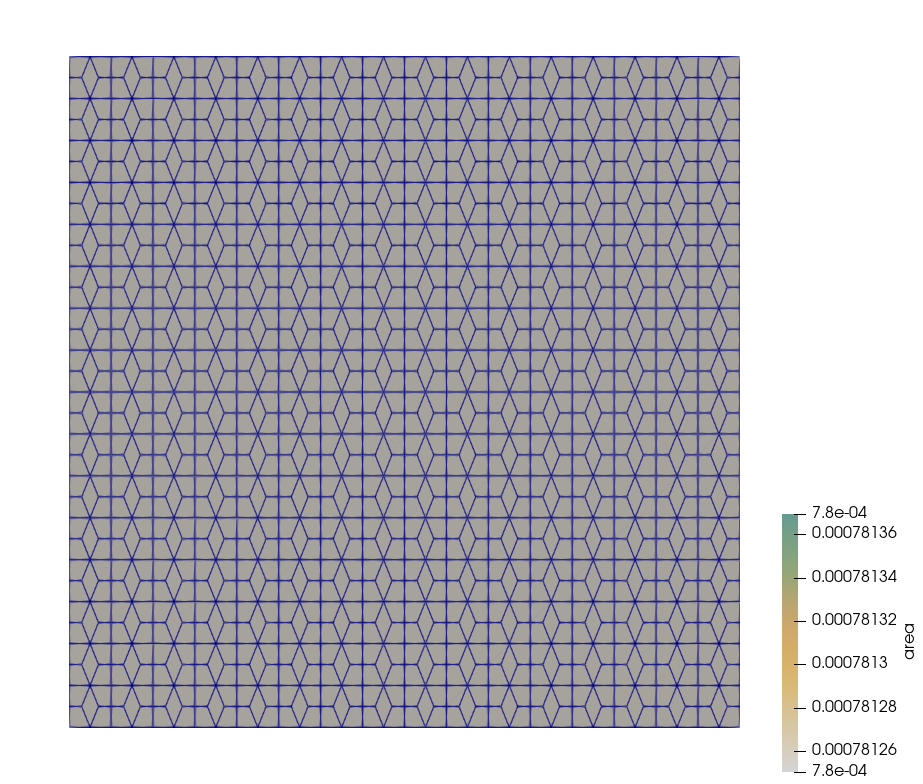
\includegraphics[width=5cm]{python_codes/fieldstone_78/images/16x16/area1.png}
\end{center}

\item the Le Tallec (LT) macro-element: it originates in \cite{leta81}. 
It is found in \cite{leru86}, \cite{qizh07}  and mentioned in \cite{brfo} and \cite{rovira1992}.
\begin{center}
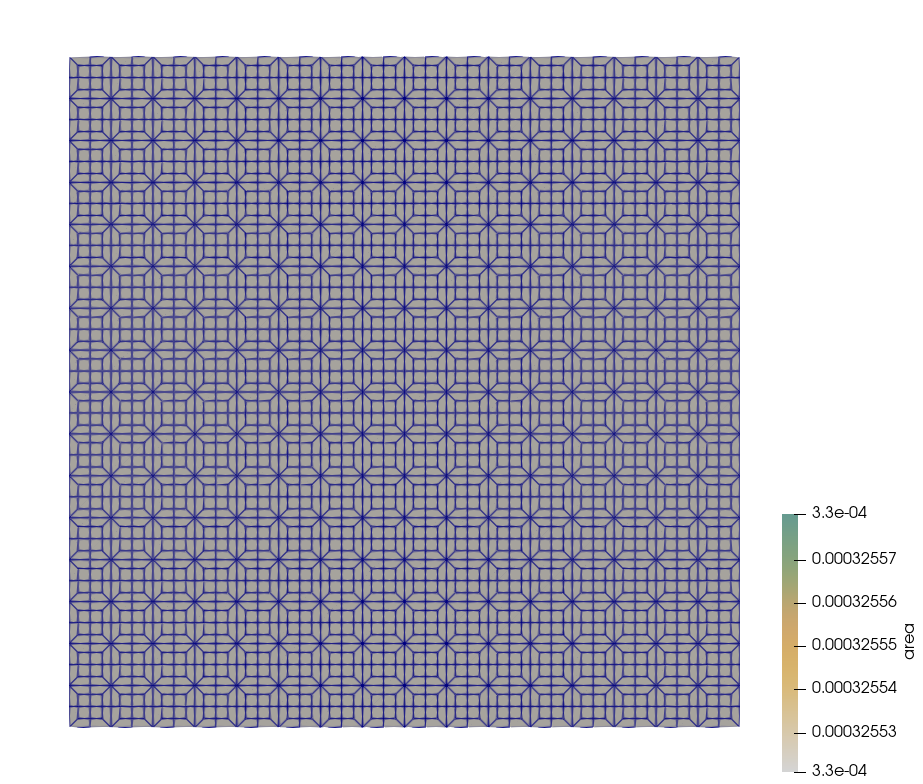
\includegraphics[width=5cm]{python_codes/fieldstone_78/images/16x16/area2.png}
\end{center}

\item the Qin \& Zhang (QZ1, QZ2, QZ3) macro-elements: they originate in \cite{qizh07}.
Note that QZ3 is in fact mentioned 2 decades before in \cite{idsn95}. See also 
remark below from \cite{rovira1992}. 
\begin{center}
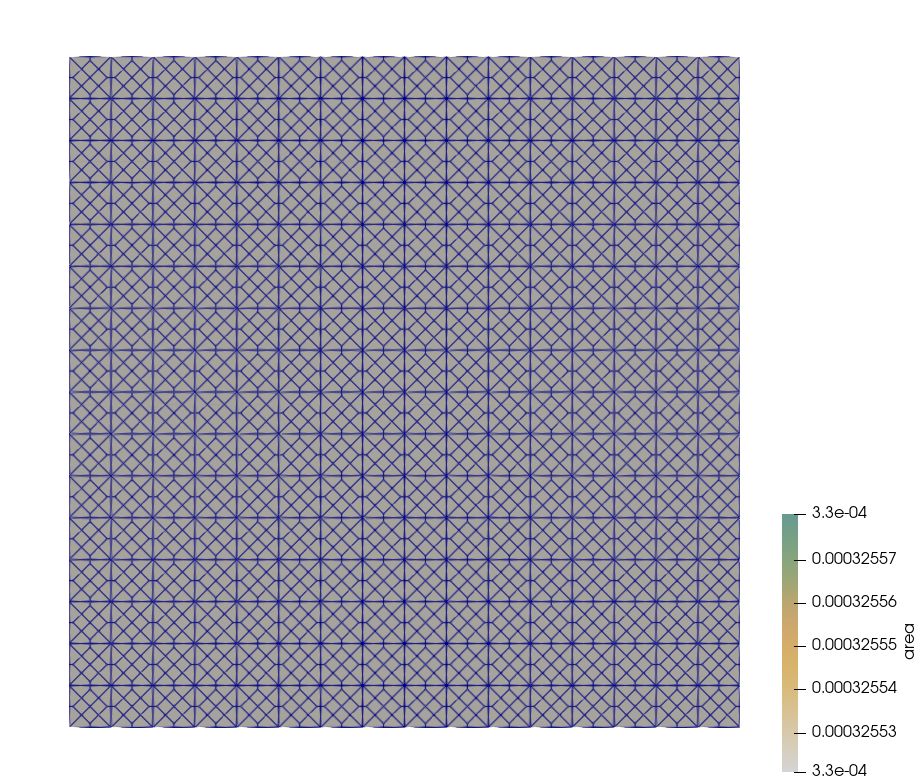
\includegraphics[width=5cm]{python_codes/fieldstone_78/images/16x16/area3.png}
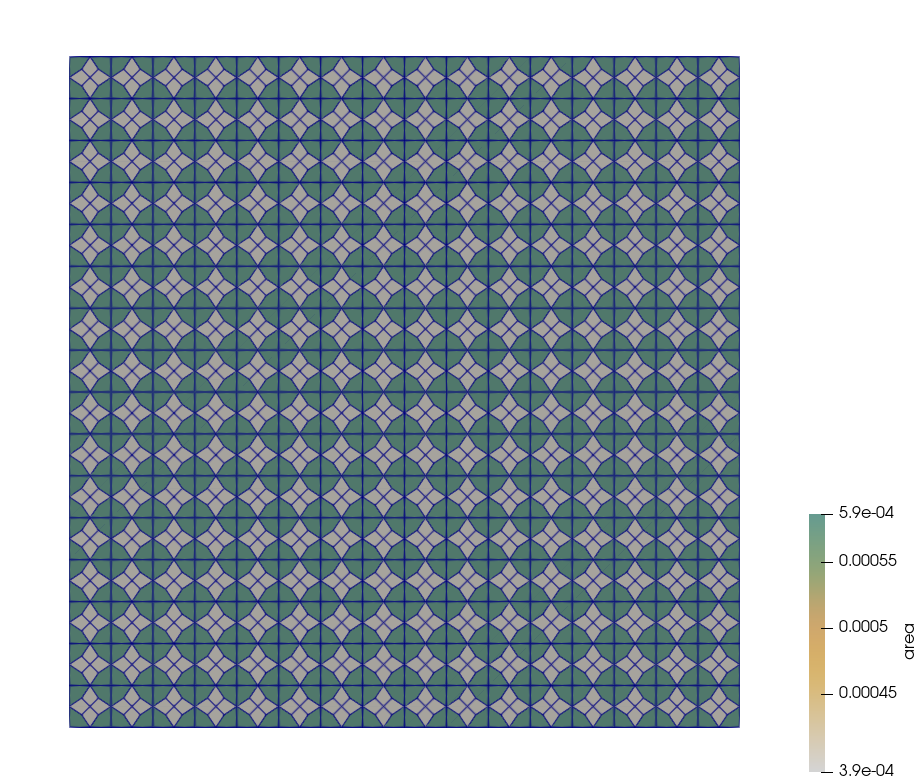
\includegraphics[width=5cm]{python_codes/fieldstone_78/images/16x16/area4.png}
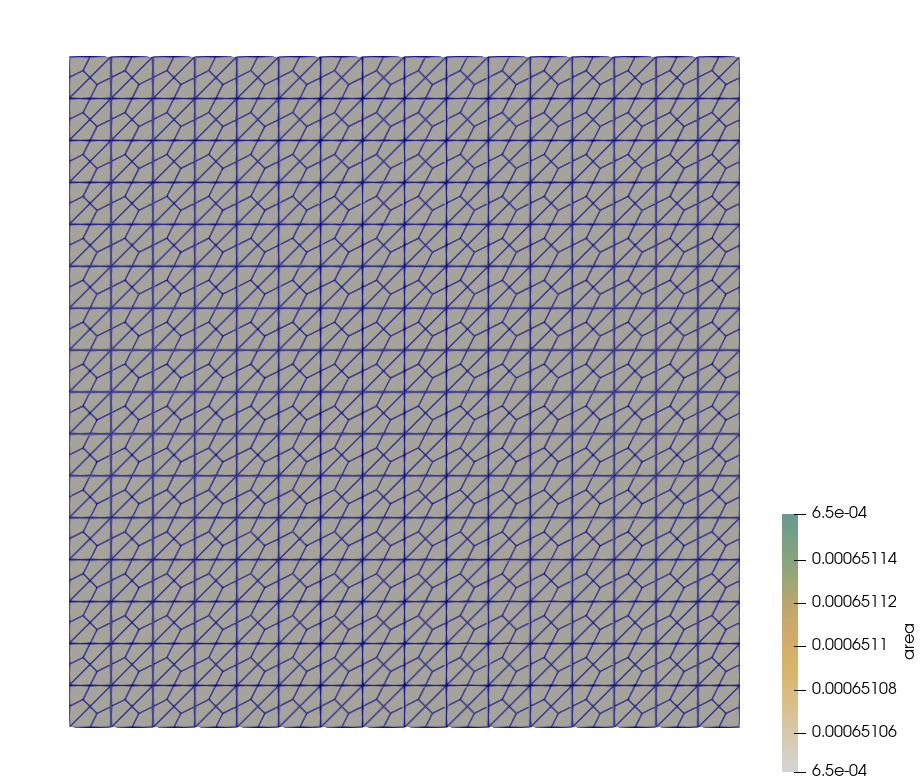
\includegraphics[width=5cm]{python_codes/fieldstone_78/images/16x16/area5.png}
\end{center}

\item mine T1, T2 

\begin{center}
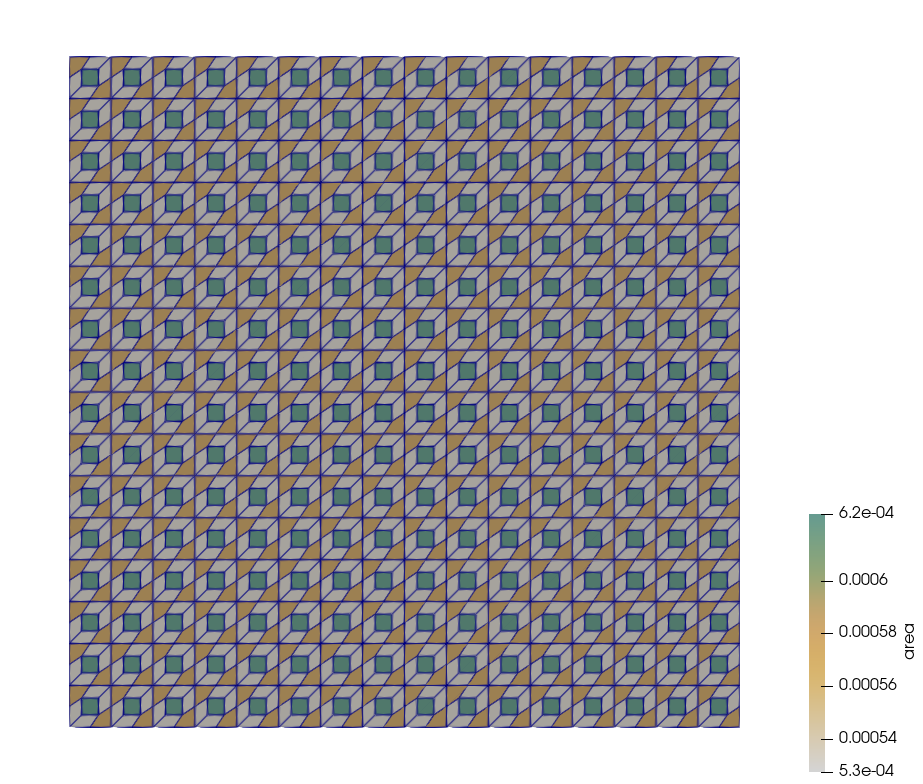
\includegraphics[width=5cm]{python_codes/fieldstone_78/images/16x16/area6.png}
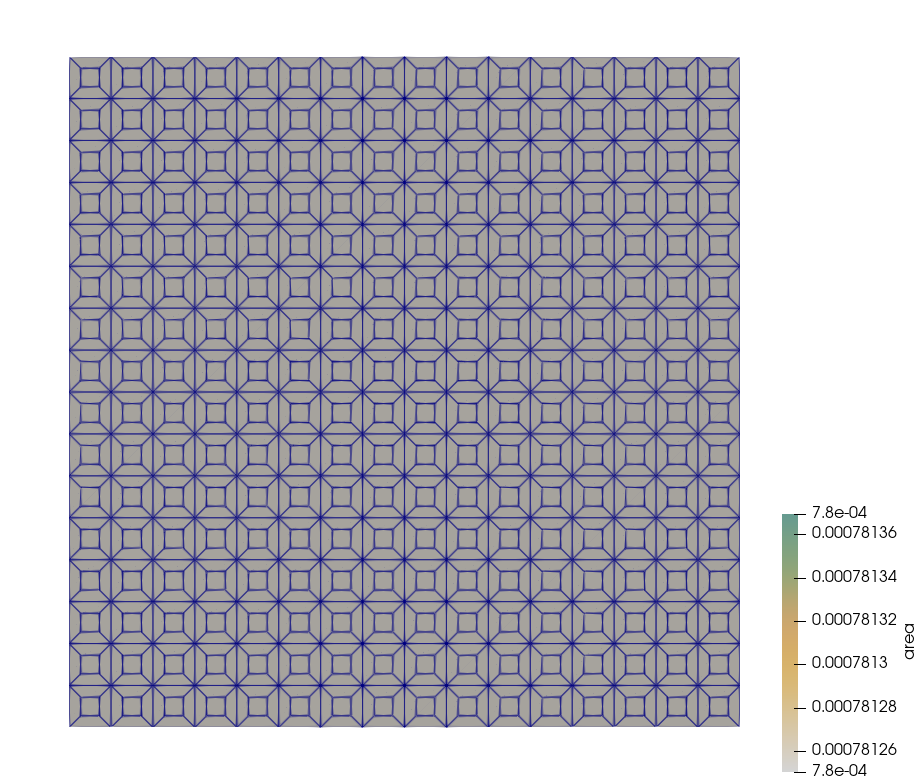
\includegraphics[width=5cm]{python_codes/fieldstone_78/images/16x16/area7.png}
\end{center}

\item RR, TR: The topology is identical to R. 
RR corresponds to moving the middle node of the macro-element by $+0.05h_x,+0.05h_y$.
TR corresponds to moving the middle node of the macro-element by $0.05\mu h_x,0.05\nu h_y$
with $\mu,\nu=-1,1$ randomly.

\begin{center}
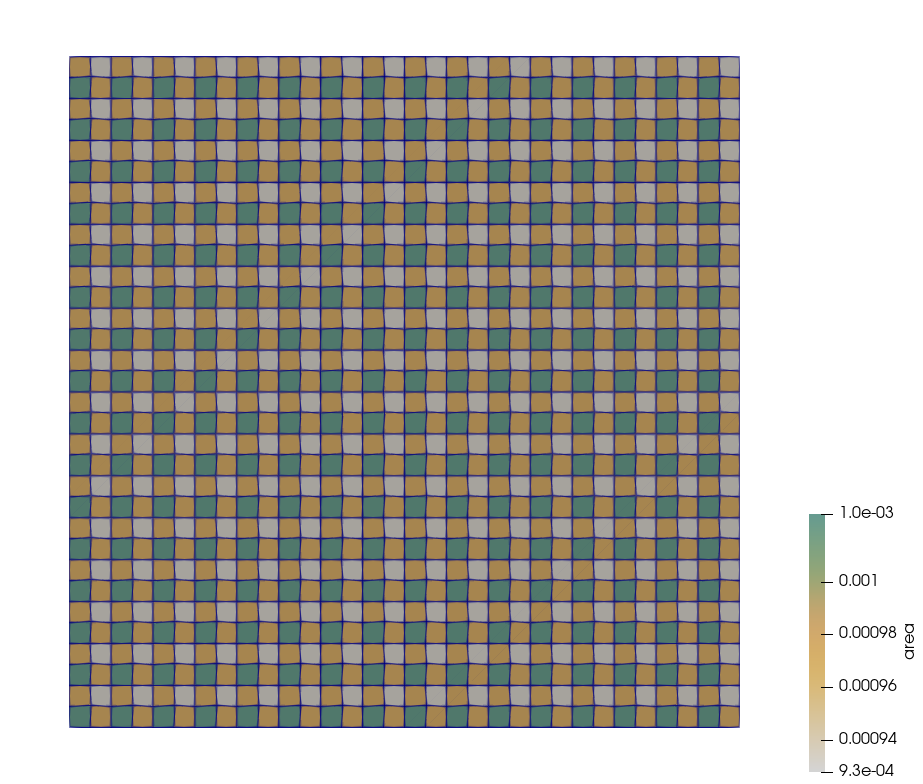
\includegraphics[width=5cm]{python_codes/fieldstone_78/images/16x16/area8.png}
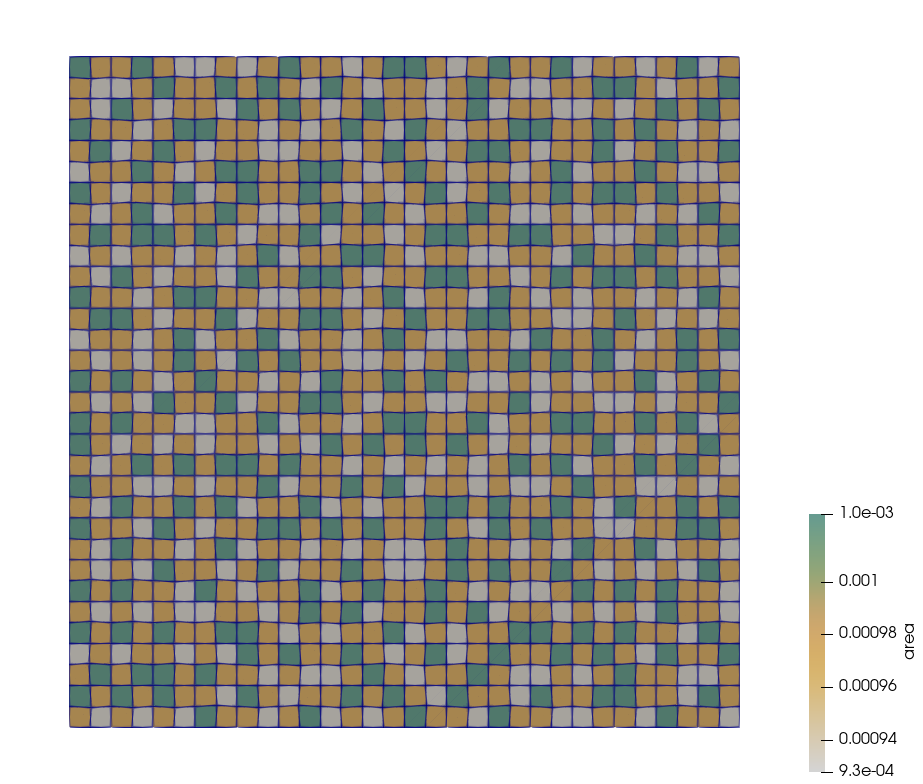
\includegraphics[width=5cm]{python_codes/fieldstone_78/images/16x16/area9.png}
\end{center}

\end{itemize}




%................................................
\paragraph{A building block for macro-elements}

We read in \textcite{rovira1992}:
\begin{displayquote}
{\color{MidnightBlue}
The velocity-constant pressure element [...] does not satisfy the BB condition, although there
are ways to stabilize it [...]. There is a simple way to see that it may work without any particular 
stabilization procedure.}

\begin{center}
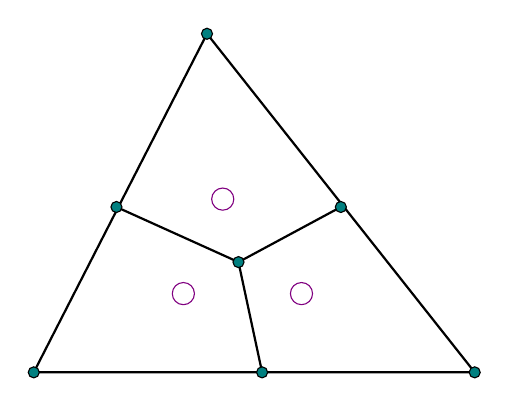
\begin{tikzpicture}
\draw[thick] (0,0) -- (5.6,0) -- (2.2,4.3)-- cycle;  
\draw[thick] (1.05,2.1) -- (2.6,1.4) -- (3.9,2.1);  
\draw[thick] (2.6,1.4) -- (2.9,0);  
\draw[black,fill=teal] (0,0) circle (2pt);
\draw[black,fill=teal] (5.6,0) circle (2pt);
\draw[black,fill=teal] (2.2,4.3) circle (2pt);
\draw[black,fill=teal] (1.05,2.1) circle (2pt);
\draw[black,fill=teal] (2.6,1.4) circle (2pt);
\draw[black,fill=teal] (3.9,2.1) circle (2pt);
\draw[black,fill=teal] (2.9,0) circle (2pt);
\draw[violet] (1.9,1) circle (4pt);
\draw[violet] (3.4,1) circle (4pt);
\draw[violet] (2.4,2.2) circle (4pt);
\end{tikzpicture}
\end{center}


{\color{MidnightBlue}
For simplicity, consider the two-dimensional case. Figure [above] shows how a quadratic
triangular element enriched with a node placed at the barycenter of the triangle can
be splitted into three bilinear elements. If we consider a pressure unknown for each
quadrilateral, we see that the velocity and pressure spaces will be isomorphic to those
of the $P_2^+ \times P_{-1}$ element [...]. The velocity-pressure interpolation for this
element satisfies the BB condition. Therefore, the macroelement depicted in [the figure above]
composed of $Q_1 \times P_0$ elements will also be div-stable.

Clearly, the main problem with this approach is the distorsion of the triangular
patch of three quadrilaterals. This patch has to be regular enough (i.e., the angles
sufficiently close to $\pi/3$) to ensure that the isoparametric mapping to the parent domain
(usually $[-1,1] \times [-1,1]$) be invertible. See Reference \cite{ciarlet2002finite} 
for the regularity conditions that a finite element partition has to satisfy.

The macroelement of [the figure above] is homeomorphic to the macroelement of Le Tallec
\& Ruas \cite{leru86}.
In the three-dimensional case, the $P_2^+ \times P_{-1}$ 
element has to be splitted into four $Q_1 \times P_0$ subelements. 
Apparently, this connexion between the $P_2^+ \times P_{-1}$ and the $Q_1 \times P_0$
elements has never been exploited.}

\end{displayquote}

We indeed find this subdivided triangle m-e in QZ1 and QZ3. 

%...................................................
\paragraph{Location of nodes inside macro element}.
When possible, we wish that all elements of a macro-element have the same area. 
For the Stenberg macro-element, we set $\delta =0.3$ (see remark at the end).
For the Le Tallex macro-element, we set $\delta=h/\sqrt{12}$ (see remark at the end).
We also make sure that all elements in QZ1,QZ3,B have same area.
However, there is a problem with QZ2: equi area yields quads with angle=$180^o$. 
Likewise macro-element T1 cannot be generated with all elements equi-area.


%................................................
\paragraph{Removal of checkerboard pattern via perturbation}

We read in \textcite{lumh24}:
\begin{displayquote}
{\color{MidnightBlue}
Griffiths and Silvester (1994) demonstrates a simple way to remove the checker-board 
error associated with the Q1-P0 element. One only needs to add a small perturbation 
to the coordinates of grid points. Here we adopt this approach in our two-phase 
implementation and perturb the coordinates of the internal vertices by 5\% of the
element size.
}
\end{displayquote}


This does not mean that it is usable with iterative solver?










%---------------------------------
\section*{Implementation}

There are 14 benchmarks/experiments that are currently implemented in the code:
\begin{enumerate}
\item Donea \& Huerta (MS) %1
\item block in the middle %2
\item sphere in the middle %3
\item aquarium %4
\item SolKz (MS) %5
\item regularised lid driven cavity %6
\item cavity (MS) %7
\item sinking block %8
\item Dohrmann \& Bochev (MS) \cite{dobo04} %9
\item flow around square cylinder % 10
\item flow over cavity % 11
\item flow over obstacle %12
\item SolCx (MS) %13
\item SolVi (MS) %14
\end{enumerate}
where MS stands for `manufactured solution'.

All experiments take place in the unit square expect experiment 8.

All experiments are isoviscous expect 3,5,8,13,14.
Note that the viscosity is evaluated in the middle of each element, not 
at the quadrature points. This can/will have an effect on non-isoviscous models.

\newpage
The meshes are created by importing the corresponding files:
\begin{lstlisting} 
import regular
import macro_S
import macro_LT
import macro_QZ1 
import macro_QZ2
import macro_QZ3
import macro_T1
import macro_T2
\end{lstlisting} 
Inside each of these files a function called {\sl mesher} is defined: 
\begin{lstlisting} 
def mesher(Lx,Ly,nelx,nely,nel,NV,mV):
\end{lstlisting} 
The arguments are the domain size $L_x$ and $L_y$, the number of macroelements
in each direction $nelx$ and $nely$, the precomputed total number of $Q_1\times P_0$ 
elements $nel$ and nodes $NV$ and the number of nodes per element $m_\upnu$.  

In what follows $p$ is the 'raw' pressure field (after normalisation)
while $q$ denotes its projection onto the nodes by means of corner-to-node average.
More specifically $q_1$ is the pressure average at the node, 
while $q_2$ is the element area weighed average
and $q_3$ is the triangle area weighed average. i.e. Scheme 2 of \cite{sagl81a}.
Note that the `filtering and smoothing' schemes proposed in this paper (section F, page 36)
are all based on the assumption
that each node belongs to four elements, which is not the case for our macro-elements here.
Interestingly \textcite{sagl81a} present their Scheme 1 as ``always successfully filters the 
CB mode, [but] cumbersome to implement''.
In practice most of the macro-elements are built so that 
the elements inside it have equal area and then $q_1=q_2=q_3$. 

Note that \textcite{sagl81a} present rules for side and corner nodes. I here do not implement these
since they would need to be adapted ad hoc for each macro-element.
See also \stone~12 about pressure smoothing.

Define errors and mesh size which is taken to be $h = \sqrt{L_xL_y/nel}$. 

%------------------------------------
\subsection*{Pressure normalization}

When it comes to the requirement of $\int_\Omega p dV=0$ we have three options
in order to enforce this constraint:
\begin{enumerate}
\item build the matrix without taking care of this constraint, and 
enforce it after the solve:
\[
\int_\Omega p dV = \sum_e A_e p_e = 0
\]
with $A_e$ being the area of element $e$.

\item Add a line and column to the matrix (Lagrange multiplier technique)
and effectively add the vector $(A_0,	 A_1, ... A_{nel-1})$ below and to the 
right of the zero pressure-pressure block of the Stokes matrix. 
The recovered pressure is then such that $sum_e A_e p_e = 0$
and the normalisation loop that comes after is useless (if only to 
verify that indeed $<p>=0$).
Post-solve normalisation is then not needed but acts as a check 
and typically returns zero (within machine precision).

\item add a line and column to the matrix that enforces $p_{nel}=0$
(or any value, really), solve the linear system and then 
normalize the pressure as in Option 1.

\end{enumerate}

Option 1 is the simplest and it works fine, except for 
experiment 9, which has a velocity field that 
does not showcases no-slip b.c.:

\begin{center}
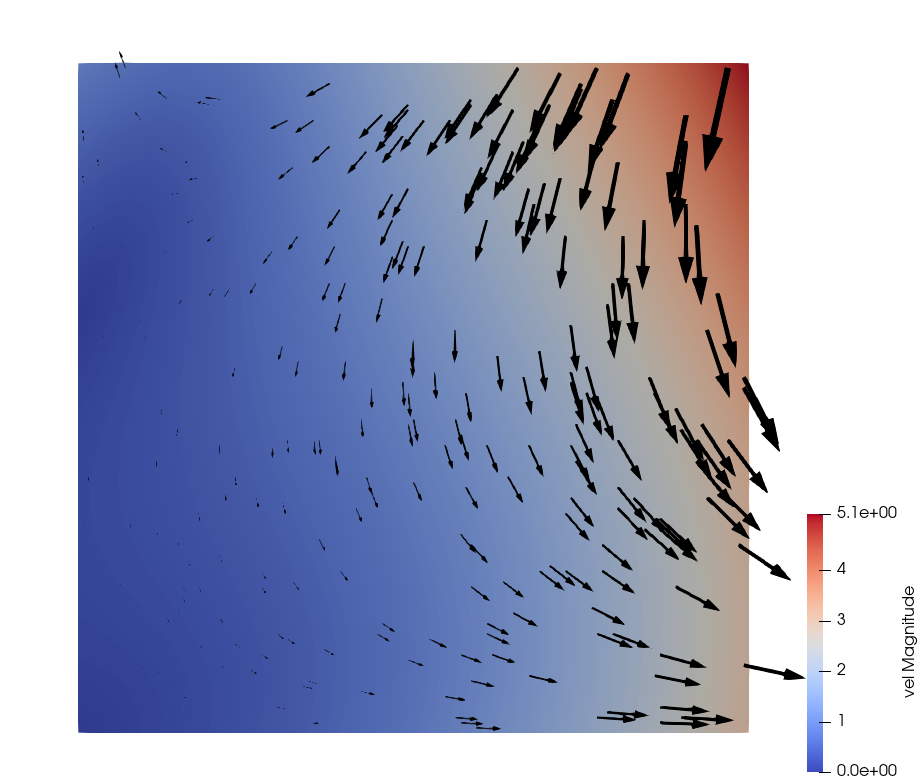
\includegraphics[width=5cm]{python_codes/fieldstone_78/results/exp09/vel.png}
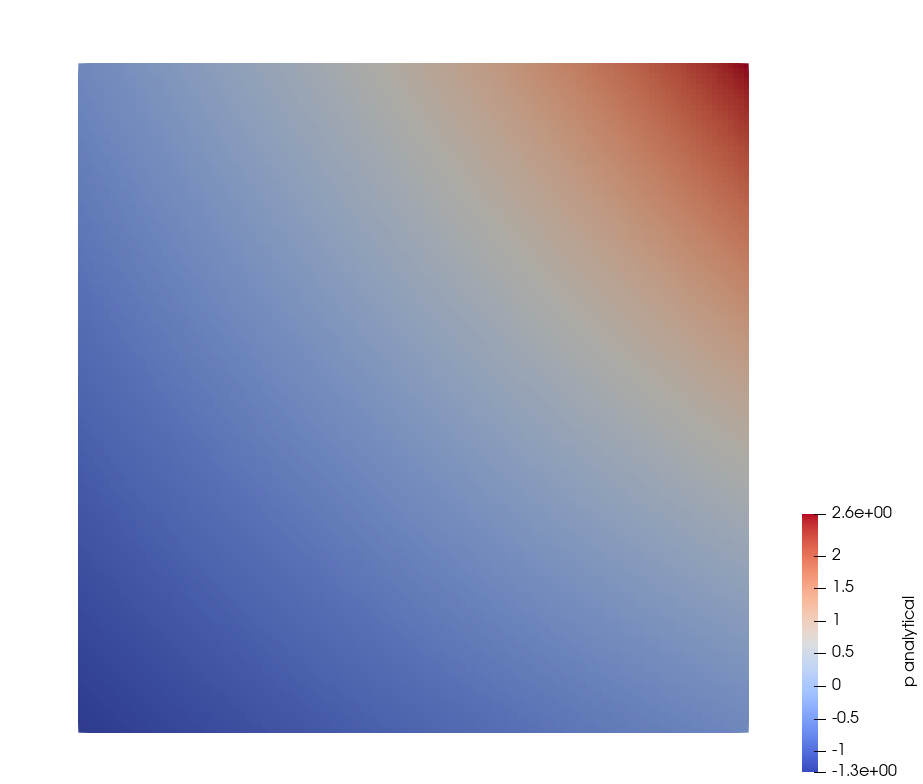
\includegraphics[width=5cm]{python_codes/fieldstone_78/results/exp09/press.png}\\
{\captionfont Experiment 9: velocity and pressure fields.}
\end{center}

I then found out that Option 2 worked {\it much} better for this experiment
and allowed to recover accurate velocities, mild pressure checkerboarding.
However the addition of the extra line probably\footnote{I cannot check this 
for sure but it makes sense -- more on this later} generated a lot of fill-ins in the direct solver
and slowed things down considerably.

\begin{center}
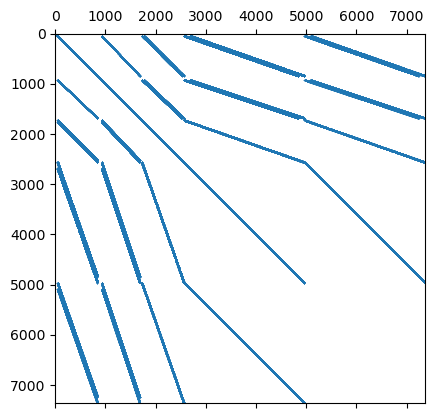
\includegraphics[width=5cm]{python_codes/fieldstone_78/images/lagrange/A_bef.png}\\
{\captionfont Example of $20\times 20$ QZ2 macro-element matrix sparsity pattern.}
\end{center}

we can verify that the three options result in the same results 
for experiment 1 for example:

{\small
\begin{verbatim}
*****Option 1*****
nel=   2400 ; errv= 0.00003035857 ; errp= 0.00419435407 ; errq1= 0.00153250868 
solve time: 0.132 s
*****Option 2*****
nel=   2400 ; errv= 0.00003035857 ; errp= 0.00419435407 ; errq1= 0.00153250868 
solve time: 1.314 s
*****Option 3*****
nel=   2400 ; errv= 0.00003035857 ; errp= 0.00419435407 ; errq1= 0.00153250868 
solve time: 0.130 s
\end{verbatim}
}

We see that Option 2 is definitely *much* slower than option 3!
and when carrying out resolution tests I found that Option 2 slowed 
the solver so much that it became unpractical. 
Also I found out that Option 2 worked but Option 3 did not (again, for experiment 9), which makes little sense. 
I then decided to follow and other lead and started to think again about the fact that 
experiment 9 showcases a non-zero flux on various faces. 

I then *suspected* that this behavior could be due to the fact 
may be there is some kind of imbalance in the overal (discrete)
flux (flow is incompressible, we should have $\int_\Gamma \vec{u}\cdot\vec{n} \; dS=0$) 
and therefore triggers extremely large insane pressure oscillations and 
yields the problem above? my instinct then tells me that 
by adding this extra line (and corresponding column) of constraints in the matrix it somewhat 
introduces some 'wiggle room' (\#technicalterm:) that compensates for the error in the b.c. imposition?

Note that in \textcite{sagl81a} we read:
`` if the imposed boundary conditions violate the constraint equation among the
normal velocities on the boundary (which again can only occur if all normal velocity
components on $\partial\Omega$ are specified), the problem is ill-posed, the algebraic system will be
inconsistent, and no solution is possible (owing to the lack of global mass balance implied by
the erroneous boundary conditions''.

Since option 2 is not an option in reality, what to do? 
For once we could start by computing the analytical flux on each face for experiment 9:
\begin{eqnarray}
\Phi_{bottom} 
&=& \int_0^1 \vec{\upnu}(x,y=0) \cdot \vec{n} \; dx \nn\\
&=& -\int_0^1 v(x,y=0)  dx \nn\\
&=& 0 \nn\\
\Phi_{top} 
&=& \int_0^1 \vec{\upnu}(x,y=1) \cdot \vec{n} \; dx \nn\\
&=& \int_0^1 v(x,y=1)  dx \nn\\
&=& \int_0^1 ( -1-2x+1 -3x^2 + 1 - x ) dx \nn\\
&=& \int_0^1 ( -3x+1 -3x^2   ) dx \nn\\
&=& -3/2 \nn\\
\Phi_{left} 
&=& \int_0^1 \vec{\upnu}(x=0,y) \cdot \vec{n} \; dy \nn\\
&=& -\int_0^1 u(x=0,y)  dy \nn\\
&=& 0 \nn\\
\Phi_{right} 
&=& \int_0^1 \vec{\upnu}(x=1,y) \cdot \vec{n} \; dy \nn\\
&=& \int_0^1 u(x=1,y)  dy \nn\\
&=& \int_0^1 (3  - y - 3y^2  ) dy \nn\\
&=& 3/2 \nn
\end{eqnarray}
And of course we find 
\[
\Phi_{total}=\Phi_{bottom}+\Phi_{top} +\Phi_{left}  + \Phi_{right}  =0
\] 
We expected this since
\[
\int_\Omega \vec{\nabla}\cdot \vec{\upnu} \; dV 
= \int_\Gamma \vec{\upnu} \cdot \vec{n} \; dS
=\Phi_{total}=\Phi_{bottom}+\Phi_{top} +\Phi_{left}  + \Phi_{right}  =0
\]

Now turning to measurements of these fluxes on each boundary,
we compute these by means of a one point quadrature on each 
element edge that is on a boundary.
The algorithm goes as follows for one of the four fluxes:
\begin{lstlisting}
flux_bottom=0
for iel in range(0,nel):
    inode0=iconV[0,iel]
    inode1=iconV[1,iel]
    inode2=iconV[2,iel]
    inode3=iconV[3,iel]
    if abs(yV[inode0]-0)/Ly<eps and abs(yV[inode1]-0)/Ly<eps:
       flux_bottom+=abs(xV[inode0]-xV[inode1])*(bc_val[inode0*ndofV+1]+bc_val[inode1*ndofV+1])/2 *-1
    if abs(yV[inode1]-0)/Ly<eps and abs(yV[inode2]-0)/Ly<eps:
       flux_bottom+=abs(xV[inode1]-xV[inode2])*(bc_val[inode1*ndofV+1]+bc_val[inode2*ndofV+1])/2 *-1
    if abs(yV[inode2]-0)/Ly<eps and abs(yV[inode3]-0)/Ly<eps:
       flux_bottom+=abs(xV[inode2]-xV[inode3])*(bc_val[inode2*ndofV+1]+bc_val[inode3*ndofV+1])/2 *-1
    if abs(yV[inode3]-0)/Ly<eps and abs(yV[inode0]-0)/Ly<eps:
       flux_bottom+=abs(xV[inode3]-xV[inode0])*(bc_val[inode3*ndofV+1]+bc_val[inode0*ndofV+1])/2 *-1
\end{lstlisting}
 
For a $32\times 32$ (R) mesh we find:
\begin{verbatim}
flux b,t,l,r= 0.0 -1.5001220703125 0.0 1.4998779296875
total_flux= -0.000244140625
\end{verbatim}
We see that the total flux is not zero (at least down to machine precision)
and this is likely to introduce a problem.

I then prescribe on the nodes of the boundary the following velocity:
\[
\vec{\upnu}^{bc} = \vec{\upnu}_{analytical} - \frac{\Phi_{measured}}{P} \vec{n}
\]
where $\Phi_{measured}$ is the measured velocity flux 
through the entire boundary and $P$ is the perimeter of the domain.
Then 
\begin{eqnarray}
\int_\Gamma \vec{\upnu}^{bc} \cdot \vec{n} \; dS
&=& \int_\Gamma \vec{\upnu}_{analytical} \cdot \vec{n} \; dS
- \int_\Gamma  \frac{\Phi_{measured}}{P} \vec{n} \cdot \vec{n} \; dS\nn\\
&=& \Phi_{measured} - \frac{\Phi_{measured}}{P} \int_\Gamma  1 \; dS \nn\\
&=& \Phi_{measured} - \frac{\Phi_{measured}}{P} P \nn\\
&=&0 \nn
\end{eqnarray}
assuming that the normal vector is a unit vector, i.e. $\vec{n}\cdot \vec{n}=1$.
I then find that applying this correction does solve the problem 
and that Option 1 is now usable again for all topologies.

Note that the problem of the normal vector at the corners does not
present itself: the quadrature points are in the middle 
of element edges and the normal vector is well defined there.

This velocity correction is transparent to all 
manufactured solutions or experiments that 
showcase free-slip or no-slip boundary conditions.

This is controled by the {\tt correct\_bcval} parameter. 

Remark: see page 291 of \textcite{vibo92} (1992).

%--------------------------------------------------------------
\subsection*{About reordering ...}

While exploring the pressure normalisation I observed that 
Option 2 was much slower than the others. I attributed this 
to the number of fill-ins generated because of the full line
added at the bottom of the pressure-pressure block. 

I then proceeded to look into reordering the complete 
Stokes matrix via the Reverse Cuthill-McKee 
algorithm\footnote{\url{https://en.wikipedia.org/wiki/Cuthill-McKee_algorithm}}
(see also \ref{MMS-ss:reordering}) which is available via SciPy:
\begin{lstlisting} 
from scipy.sparse.csgraph import reverse_cuthill_mckee
\end{lstlisting} 
Once the matrix is fully assembled I use the 'spy' function 
to generate a plot of its sparsity patten.
I then proceed to use the RCM algorithm as follows:
\begin{lstlisting} 
if apply_RCM:
   perm=reverse_cuthill_mckee(A_csr,symmetric_mode=True)
   perm_inv=np.empty(len(perm),dtype=np.int32)
   for i in range(0,len(perm)):
       perm_inv[perm[i]]=i
   A_csr=A_csr[np.ix_(perm,perm)]
   rhs=rhs[np.ix_(perm)]
\end{lstlisting} 
Another snapshot of the matrix is then produced after the reordering. 
Before and after snapshots are shown below for all 8 topologies 
(in the absence of any pressure normalisation Lagrange multiplier line):

\begin{center}
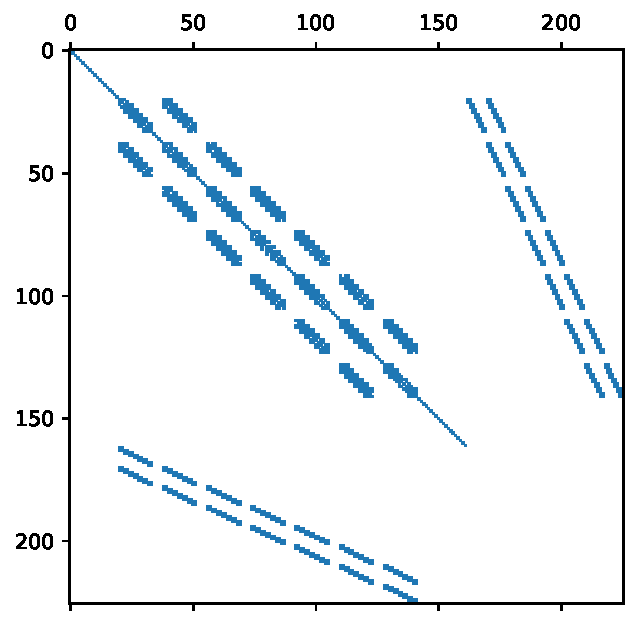
\includegraphics[width=4cm]{python_codes/fieldstone_78/results/spy/A_bef_topo0.pdf}
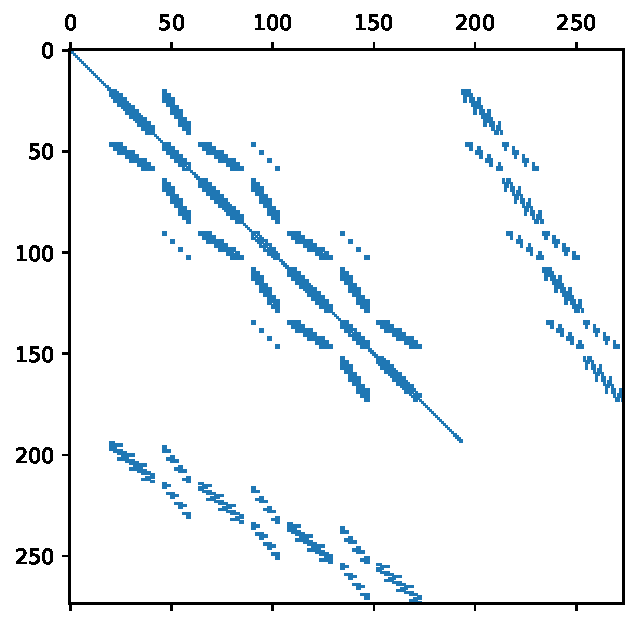
\includegraphics[width=4cm]{python_codes/fieldstone_78/results/spy/A_bef_topo1.pdf}
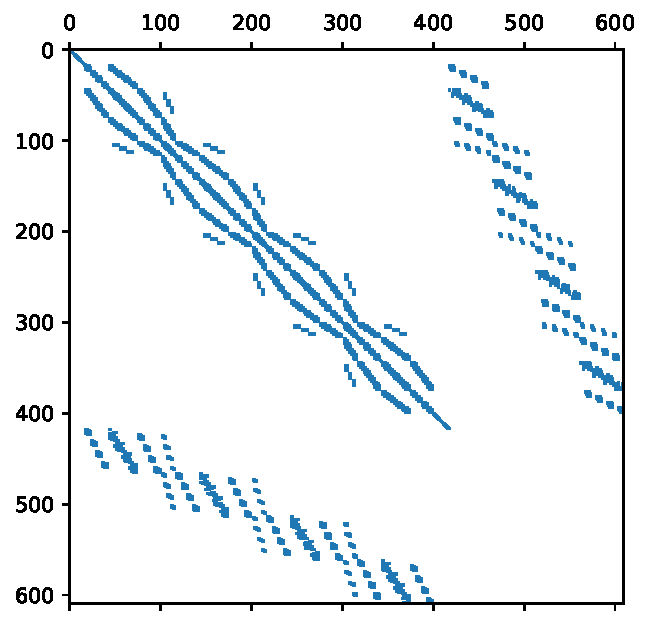
\includegraphics[width=4cm]{python_codes/fieldstone_78/results/spy/A_bef_topo2.pdf}
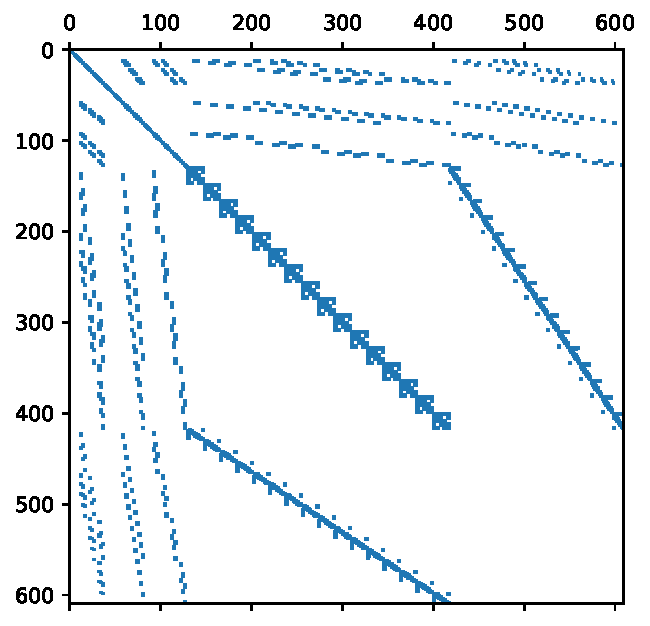
\includegraphics[width=4cm]{python_codes/fieldstone_78/results/spy/A_bef_topo3.pdf}\\
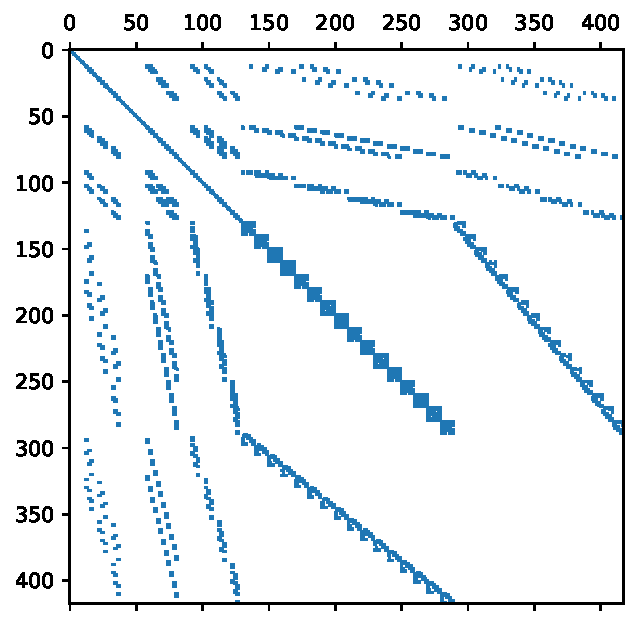
\includegraphics[width=4cm]{python_codes/fieldstone_78/results/spy/A_bef_topo4.pdf}
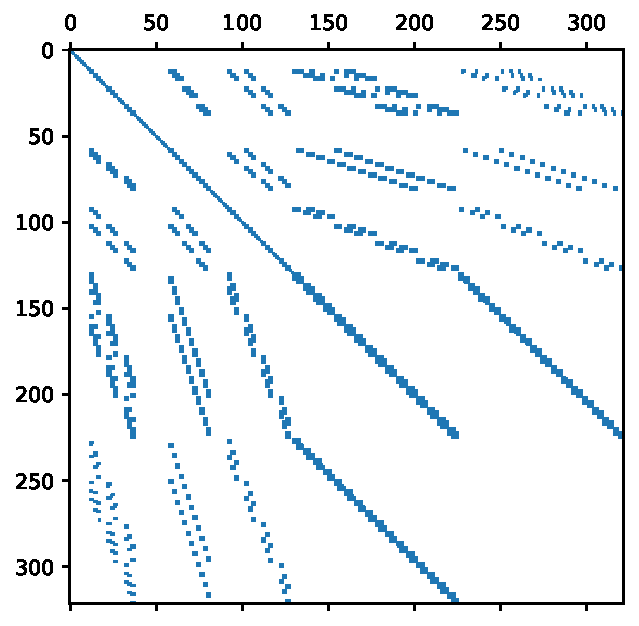
\includegraphics[width=4cm]{python_codes/fieldstone_78/results/spy/A_bef_topo5.pdf}
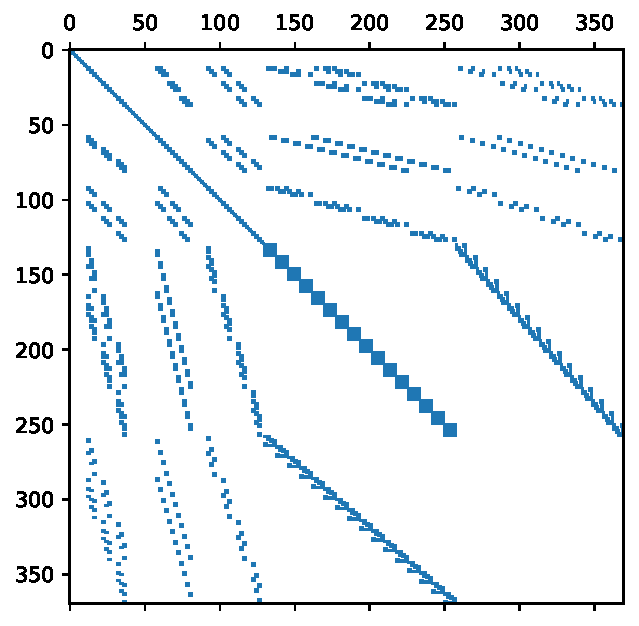
\includegraphics[width=4cm]{python_codes/fieldstone_78/results/spy/A_bef_topo6.pdf}
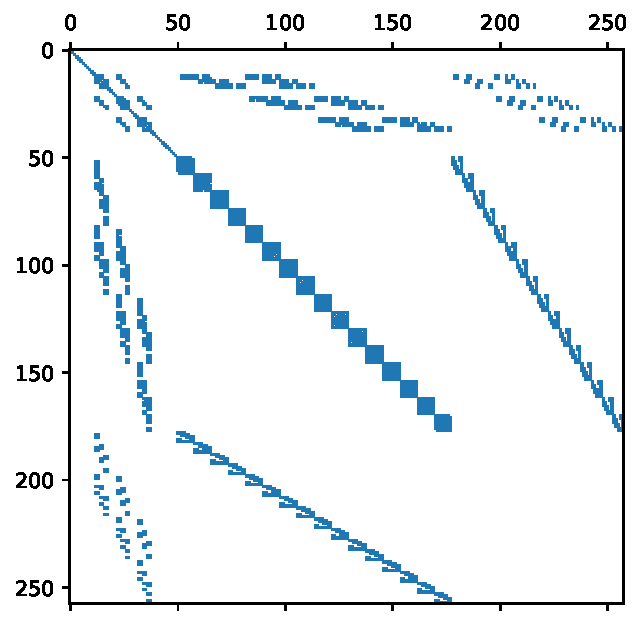
\includegraphics[width=4cm]{python_codes/fieldstone_78/results/spy/A_bef_topo7.pdf}\\
{\captionfont Before: 4x4 macro-element mesh}
\end{center}

\begin{center}
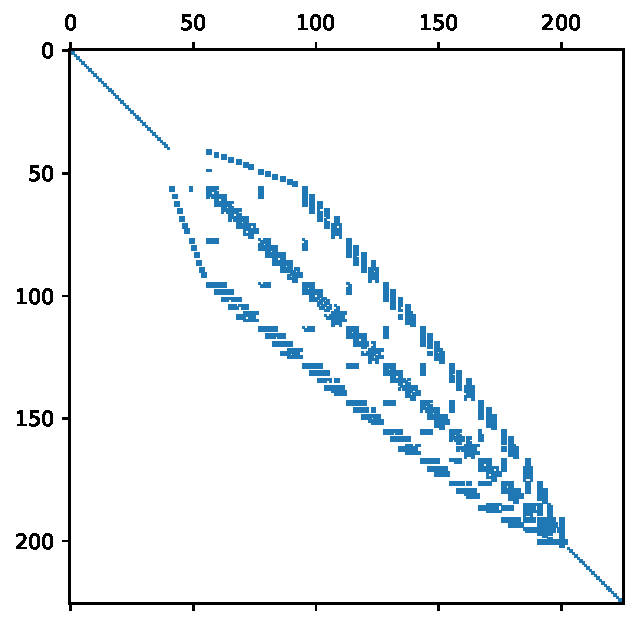
\includegraphics[width=4cm]{python_codes/fieldstone_78/results/spy/A_aft_topo0.pdf}
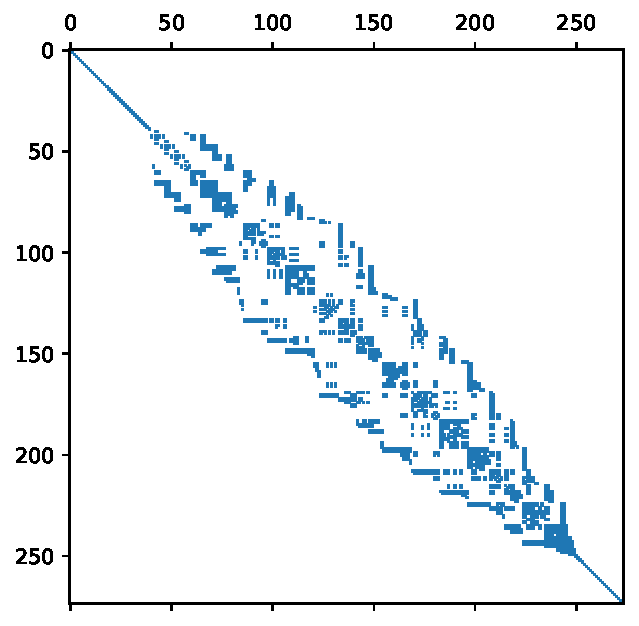
\includegraphics[width=4cm]{python_codes/fieldstone_78/results/spy/A_aft_topo1.pdf}
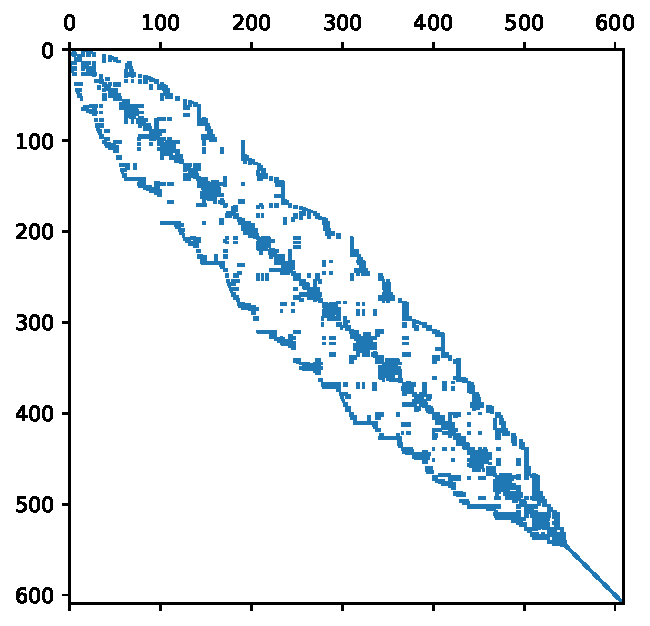
\includegraphics[width=4cm]{python_codes/fieldstone_78/results/spy/A_aft_topo2.pdf}
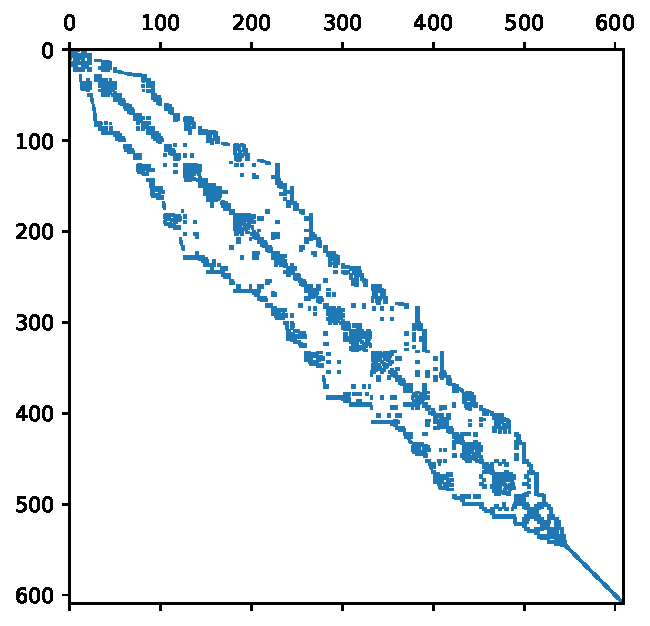
\includegraphics[width=4cm]{python_codes/fieldstone_78/results/spy/A_aft_topo3.pdf}\\
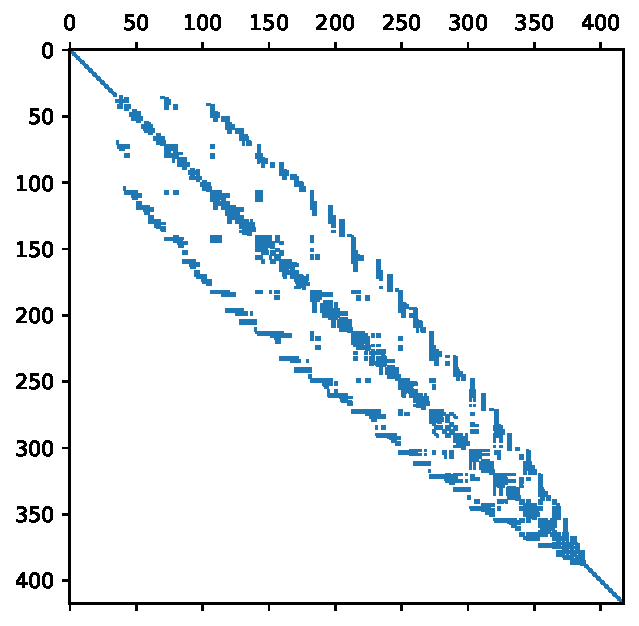
\includegraphics[width=4cm]{python_codes/fieldstone_78/results/spy/A_aft_topo4.pdf}
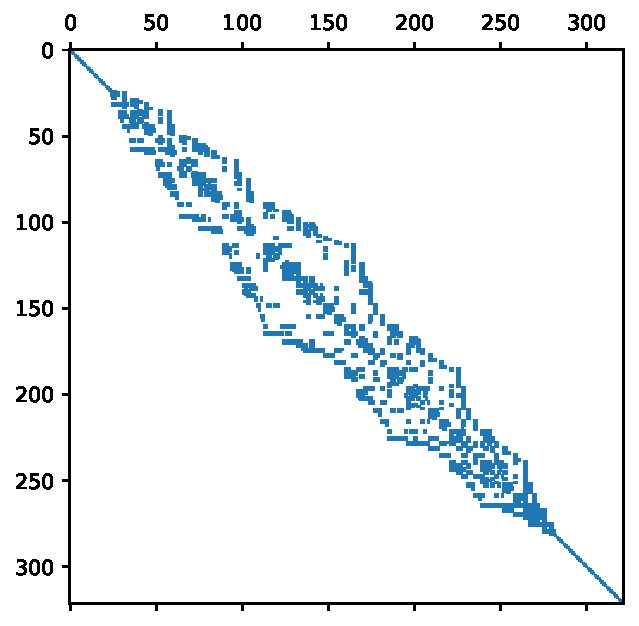
\includegraphics[width=4cm]{python_codes/fieldstone_78/results/spy/A_aft_topo5.pdf}
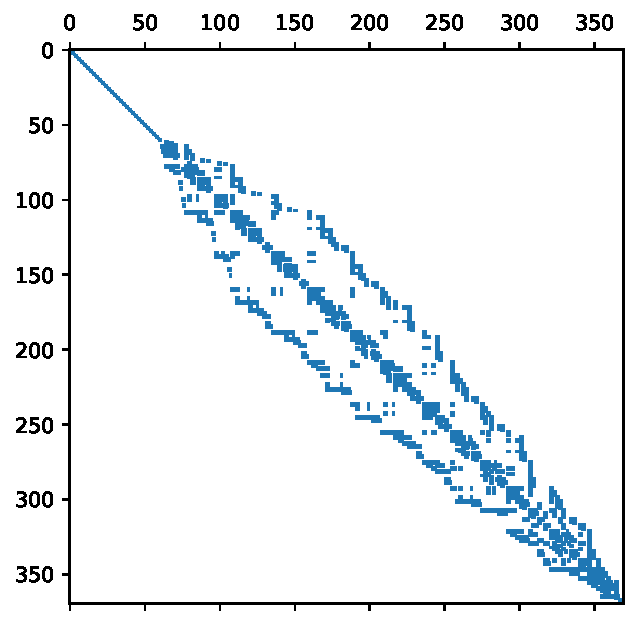
\includegraphics[width=4cm]{python_codes/fieldstone_78/results/spy/A_aft_topo6.pdf}
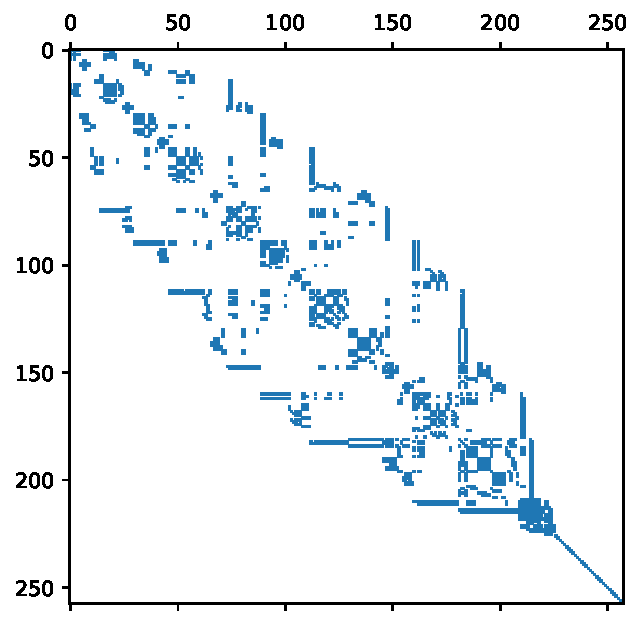
\includegraphics[width=4cm]{python_codes/fieldstone_78/results/spy/A_aft_topo7.pdf}\\
{\captionfont After: 4x4 macro-element mesh}
\end{center}

After the solve, the solution vector must be reordered to 
comply with the connectivity array:
\begin{lstlisting} 
if apply_RCM:
   sol=sol[np.ix_(perm_inv)]
\end{lstlisting} 















\newpage
%-----------------------------------------------------------------
\subsection*{Testing for the existence of checkerboard modes}



\[
\G_{el} = -\int_{\Omega_e} {\bm B}^T \cdot {\bm N} dV
= -\int_{\Omega_e}
\left(
\begin{array}{ccc}
\partial_x \bN_1^\upnu & 0 & \partial_y \bN_1^\upnu \\
0 & \partial_y \bN_1^\upnu & \partial_x \bN_1^\upnu \\
\partial_x \bN_2^\upnu & 0 & \partial_y \bN_2^\upnu \\
0 & \partial_y \bN_2^\upnu & \partial_x \bN_2^\upnu \\
\dots & \dots & \dots \\
\dots & \dots & \dots \\
\partial_x \bN_{m_\upnu}^\upnu & 0 & \partial_y \bN_{m_\upnu}^\upnu \\
0 & \partial_y \bN_{m_\upnu}^\upnu & \partial_x \bN_{m_\upnu}^\upnu 
\end{array}
\right)
\cdot
\left(
\begin{array}{cccc}
\bN_1^p & \bN_2^p & \dots & \bN_{m_p}^p \\ 
\bN_1^p & \bN_2^p & \dots & \bN_{m_p}^p \\ 
0 & 0 & \dots & 0
\end{array}
\right)
dV
\]
Since we are dealing with $Q_1\times P_0$ elements then $m_p=1$ and $\bN^p(x,y)=1$.
This yields
\[
\G_{el} = -\int_{\Omega_e} {\bm B}^T \cdot {\bm N} dV
= -\int_{\Omega_e}
\left(
\begin{array}{ccc}
\partial_x \bN_1^\upnu \\
\partial_y \bN_1^\upnu \\
\partial_x \bN_2^\upnu \\
\partial_y \bN_2^\upnu \\
\partial_x \bN_3^\upnu \\
\partial_y \bN_3^\upnu \\
\partial_x \bN_4^\upnu \\
\partial_y \bN_4^\upnu 
\end{array}
\right)
dV
\]

In what follows we proceed to build the assembled block $\G$ for each macro element, 
impose no slip boundary conditions on all sides (thereby zeroing many lines of the
matrix), and compute the null space of the remaining lines. 
Ideally only one pressure solution should be in the null space, the space of 
all constant vectors since then $\G \cdot \vec{\cal P}=\vec{0}$.
If/when the nullspace is larger than one, then checkerboard patterns (aka 
spurious modes) can exist and degrade the solution. 

This study can be carried out by setting the \lstinline{nullspace} parameter to 
\lstinline{True} and the number of elements and domain size is then set automatically.

\newpage
The 8 macro-elements considered here are shown hereunder 
with their internal numbering of nodes:

\begin{center}
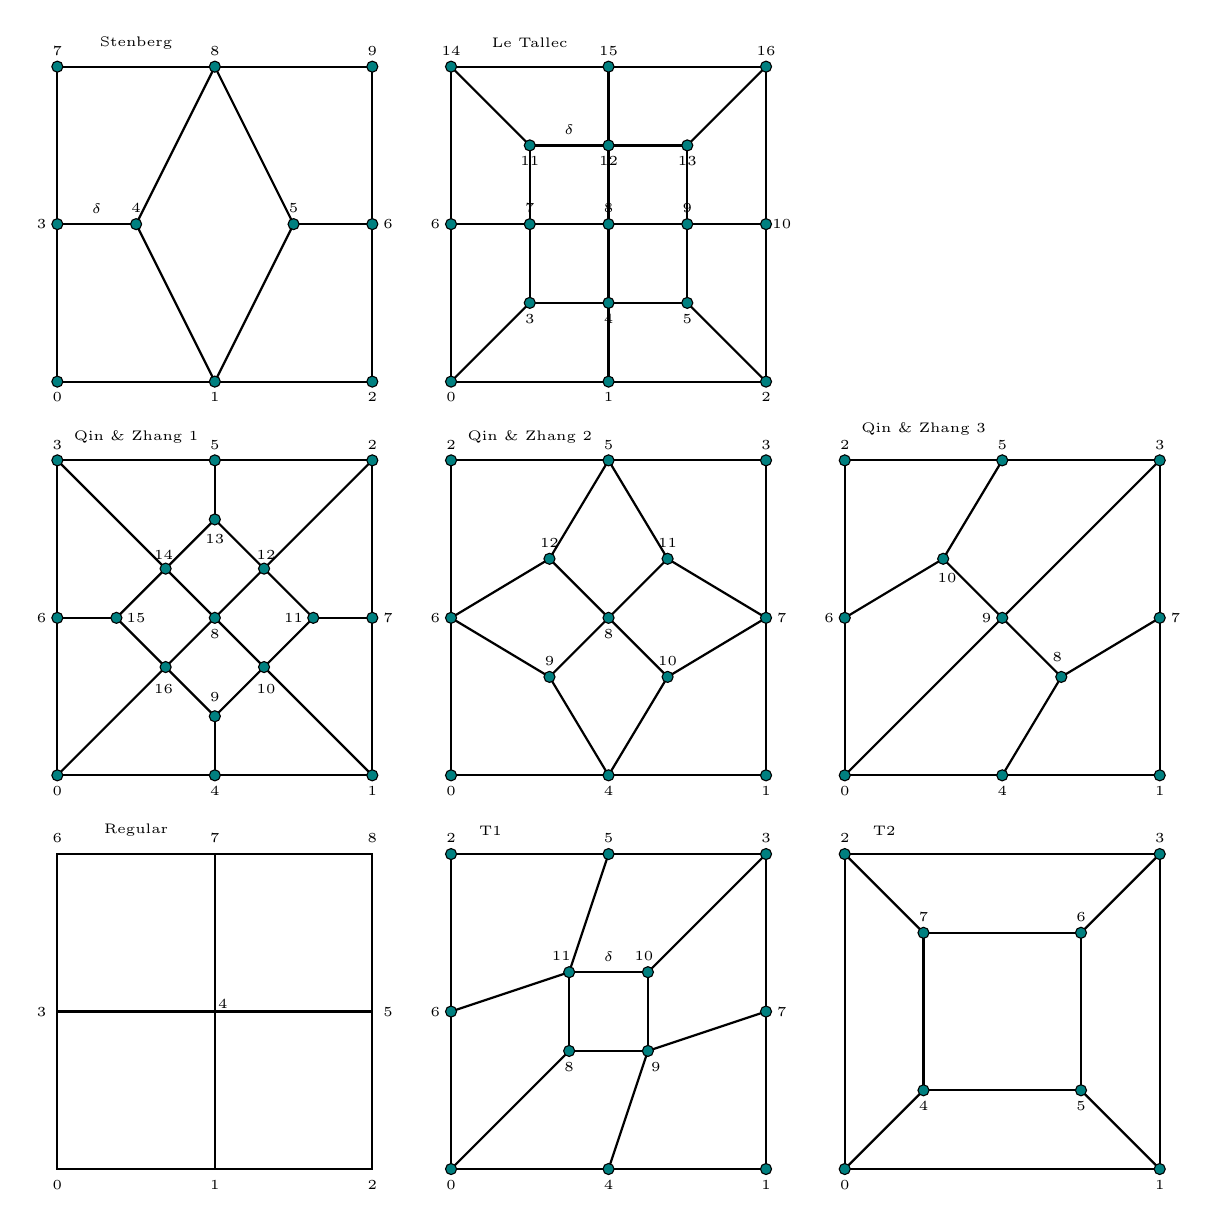
\begin{tikzpicture}
%\draw[fill=gray!23,gray!23](0,0) rectangle (15,15);
%\draw[step=0.5cm,gray,very thin] (0,0) grid (15,15); %background grid


%%%%%%%%%%%%%%%%%%%%%%%%%%%%%%%%%%%%%%%%%%%%%%%%%%%%%%%%%%%%%%%%%%
%stenberg
\node[] at (1,14.3) {\tiny Stenberg};
\draw[thick] (0,10) -- (4,10) -- (4,14) -- (0,14) -- cycle;  
\draw[thick] (2,10) -- (3,12) -- (2,14) -- (1,12) -- cycle;  
\draw[thick] (0,12) -- (1,12);  
\draw[thick] (3,12) -- (4,12);  
\draw[black,fill=teal] (0,10) circle (2pt);
\draw[black,fill=teal] (4,10) circle (2pt);
\draw[black,fill=teal] (4,14) circle (2pt);
\draw[black,fill=teal] (0,14) circle (2pt);
\draw[black,fill=teal] (2,10) circle (2pt);
\draw[black,fill=teal] (2,14) circle (2pt);
\draw[black,fill=teal] (0,12) circle (2pt);
\draw[black,fill=teal] (4,12) circle (2pt);
\draw[black,fill=teal] (1,12) circle (2pt);
\draw[black,fill=teal] (3,12) circle (2pt);

\node[] at (0,10-0.2) {\tiny 0};
\node[] at (4,10-0.2) {\tiny 2};
\node[] at (4,14+0.2) {\tiny 9};
\node[] at (0,14+0.2) {\tiny 7};
\node[] at (2,10-0.2) {\tiny 1};
\node[] at (2,14+0.2) {\tiny 8};
\node[] at (0-0.2,12) {\tiny 3};
\node[] at (4+0.2,12) {\tiny 6};
\node[] at (1,12+0.2) {\tiny 4};
\node[] at (3,12+0.2) {\tiny 5};


\node[] at (0.5,12.2) {\tiny $\delta$};

%%%%%%%%%%%%%%%%%%%%%%%%%%%%%%%%%%%%%%%%%%%%%%%%%%%%%%%%%%%%%%%%%%%
%letallec
\node[] at (6,14.3) {\tiny Le Tallec};
\draw[thick] (5,10) -- (9,10) -- (9,14) -- (5,14) -- cycle;  
\draw[thick] (6,11) -- (8,11) -- (8,13) -- (6,13) -- cycle;  
\draw[thick] (5,10) -- (6,11) ;  
\draw[thick] (9,10) -- (8,11) ;  
\draw[thick] (9,14) -- (8,13) ;  
\draw[thick] (5,14) -- (6,13) ;  
\draw[thick] (5,12) -- (9,12) ;  
\draw[thick] (7,10) -- (7,14) ;  
\draw[black,fill=teal] (0+5,10) circle (2pt);
\draw[black,fill=teal] (4+5,10) circle (2pt);
\draw[black,fill=teal] (4+5,14) circle (2pt);
\draw[black,fill=teal] (0+5,14) circle (2pt);
\draw[black,fill=teal] (6,11) circle (2pt);
\draw[black,fill=teal] (8,11) circle (2pt);
\draw[black,fill=teal] (8,13) circle (2pt);
\draw[black,fill=teal] (6,13) circle (2pt);
\draw[black,fill=teal] (7,10) circle (2pt);
\draw[black,fill=teal] (5,12) circle (2pt);
\draw[black,fill=teal] (9,12) circle (2pt);
\draw[black,fill=teal] (7,14) circle (2pt);
\draw[black,fill=teal] (6,12) circle (2pt);
\draw[black,fill=teal] (7,12) circle (2pt);
\draw[black,fill=teal] (8,12) circle (2pt);
\draw[black,fill=teal] (7,11) circle (2pt);
\draw[black,fill=teal] (7,13) circle (2pt);


\node[] at (0+5,10-0.2) {\tiny 0};
\node[] at (2+5,10-0.2) {\tiny 1};
\node[] at (4+5,10-0.2) {\tiny 2};
\node[] at (1+5,11-0.2) {\tiny 3};
\node[] at (2+5,11-0.2) {\tiny 4};
\node[] at (3+5,11-0.2) {\tiny 5};
\node[] at (0-0.2+5,12) {\tiny 6};
\node[] at (1+5,12+0.2) {\tiny 7};
\node[] at (2+5,12+0.2) {\tiny 8};
\node[] at (3+5,12+0.2) {\tiny 9};
\node[] at (4+0.2+5,12) {\tiny 10};
\node[] at (1+5,13-0.2) {\tiny 11};
\node[] at (2+5,13-0.2) {\tiny 12};
\node[] at (3+5,13-0.2) {\tiny 13};
\node[] at (0+5,14+0.2) {\tiny 14};
\node[] at (2+5,14+0.2) {\tiny 15};
\node[] at (4+5,14+0.2) {\tiny 16};

\node[] at (6.5,13.2) {\tiny $\delta$};

%%%%%%%%%%%%%%%%%%%%%%%%%%%%%%%%%%%%%%%%%%%%%%%%%%%%%%%%%%%%%%%%%%
%qizh1
\node[] at (1,9.3) {\tiny Qin \& Zhang 1};

\draw[thick] (0,5) -- (4,5) -- (4,9) -- (0,9) -- cycle;  
\draw[thick] (1.75-1,3+4) -- (3-1,1.75+4) -- (4.25-1,3+4) -- (3-1,4.25+4) -- cycle;  
\draw[thick] (1-1,1+4) -- (5-1,5+4) ;  
\draw[thick] (1-1,5+4) -- (5-1,1+4) ;  
\draw[thick] (3-1,1+4) -- (3-1,1.75+4) ;  
\draw[thick] (3-1,4.25+4) -- (3-1,5+4) ;  
\draw[thick] (1-1,3+4) -- (1.75-1,3+4) ;  
\draw[thick] (4.25-1,3+4) -- (5-1,3+4) ;  
\draw[black,fill=teal] (1-1,1+4)   circle (2pt);
\draw[black,fill=teal] (3-1,1+4)   circle (2pt);
\draw[black,fill=teal] (5-1,1+4)   circle (2pt);

\draw[black,fill=teal] (3-1,1.75+4)   circle (2pt);
\draw[black,fill=teal] (2.375-1,2.375+4)   circle (2pt);
\draw[black,fill=teal] (3.625-1,2.375+4)   circle (2pt);

\draw[black,fill=teal] (1-1,3+4)   circle (2pt);
\draw[black,fill=teal] (1.75-1,3+4)   circle (2pt);
\draw[black,fill=teal] (3-1,3+4)   circle (2pt);
\draw[black,fill=teal] (4.25-1,3+4)   circle (2pt);
\draw[black,fill=teal] (5-1,3+4)   circle (2pt);

\draw[black,fill=teal] (2.375-1,3.625+4)   circle (2pt);
\draw[black,fill=teal] (3.625-1,3.625+4)   circle (2pt);
\draw[black,fill=teal] (3-1,4.25+4)   circle (2pt);

\draw[black,fill=teal] (1-1,5+4)   circle (2pt);
\draw[black,fill=teal] (3-1,5+4)   circle (2pt);
\draw[black,fill=teal] (5-1,5+4)   circle (2pt);


\node[] at (0,5-0.2) {\tiny 0};
\node[] at (2,5-0.2) {\tiny 4};
\node[] at (4,5-0.2) {\tiny 1};
\node[] at (0-0.2,7) {\tiny 6};
\node[] at (1,7) {\tiny 15};
\node[] at (2,7-0.2) {\tiny 8};
\node[] at (3,7) {\tiny 11};
\node[] at (4+0.2,7) {\tiny 7};
\node[] at (2,6) {\tiny 9};
\node[] at (2,8) {\tiny 13};
\node[] at (0,9+0.2) {\tiny 3};
\node[] at (2,9+0.2) {\tiny 5};
\node[] at (4,9+0.2) {\tiny 2};

\node[] at (1.35,6.1) {\tiny 16};
\node[] at (2.65,6.1) {\tiny 10};
\node[] at (1.35,7.8) {\tiny 14};
\node[] at (2.65,7.8) {\tiny 12};



%%%%%%%%%%%%%%%%%%%%%%%%%%%%%%%%%%%%%%%%%%%%%%%%%%%%%%%%%%%%%
\draw[thick] (5,5) -- (9,5) -- (9,9) -- (5,9) -- cycle;  
\node[] at (6,9.3) {\tiny Qin \& Zhang 2};

\draw[thick] (1+4,3+4) -- (2.25+4,2.25+4) -- (3+4,1+4) -- (3.75+4,2.25+4) -- (5+4,3+4) --(3.75+4,3.75+4) -- (3+4,5+4) --(2.25+4,3.75+4) --cycle;  
\draw[thick] (2.25+4,2.25+4) -- (3.75+4,3.75+4) ;  %diags
\draw[thick] (2.25+4,3.75+4) -- (3.75+4,2.25+4) ;  

\draw[black,fill=teal] (1+4,1+4)   circle (2pt); %perimeter nodes
\draw[black,fill=teal] (3+4,1+4)   circle (2pt);
\draw[black,fill=teal] (5+4,1+4)   circle (2pt);
\draw[black,fill=teal] (1+4,3+4)   circle (2pt);
\draw[black,fill=teal] (3+4,3+4)   circle (2pt);
\draw[black,fill=teal] (5+4,3+4)   circle (2pt);
\draw[black,fill=teal] (1+4,5+4)   circle (2pt);
\draw[black,fill=teal] (3+4,5+4)   circle (2pt);
\draw[black,fill=teal] (5+4,5+4)   circle (2pt);

\draw[black,fill=teal] (2.25+4,2.25+4)   circle (2pt); %inside nodes
\draw[black,fill=teal] (3.75+4,3.75+4)   circle (2pt);
\draw[black,fill=teal] (2.25+4,3.75+4)   circle (2pt);
\draw[black,fill=teal] (3.75+4,2.25+4)   circle (2pt);


\node[] at (1+4,1+4-0.2) {\tiny 0};
\node[] at (1+6,1+4-0.2) {\tiny 4};
\node[] at (1+8,1+4-0.2) {\tiny 1};
\node[] at (1+4-0.2,1+6) {\tiny 6};
\node[] at (1+6,1+6-0.2) {\tiny 8};
\node[] at (1+8+0.2,1+6) {\tiny 7};
\node[] at (1+4,1+8+0.2) {\tiny 2};
\node[] at (1+6,1+8+0.2) {\tiny 5};
\node[] at (1+8,1+8+0.2) {\tiny 3};
\node[] at (2.25+4,2.25+4+0.2) {\tiny 9};
\node[] at (2.25+4+1.5,2.25+4+0.2) {\tiny 10};
\node[] at (2.25+4,2.25+4+1.5+0.2) {\tiny 12};
\node[] at (2.25+4+1.5,2.25+4+1.5+0.2) {\tiny 11};


%%%%%%%%%%%%%%%%%%%%%%%%%%%%%%%%%%%%%%%%%%%%%%%%%%%%%%%%%%%%%
\node[] at (11,9.4) {\tiny Qin \& Zhang 3};
\draw[thick] (10,5) -- (14,5) -- (14,9) -- (10,9) -- cycle;  

\draw[thick] (1+9,3+4) -- (2.25+9,3.75+4) -- (3+9,5+4);
\draw[thick] (3+9,1+4) -- (3.75+9,2.25+4) -- (5+9,3+4);
\draw[thick] (1+9,1+4) -- (5+9,5+4) ;  %diags
\draw[thick] (2.25+9,3.75+4) -- (3.75+9,2.25+4) ;  

\draw[black,fill=teal] (1+9,1+4)   circle (2pt); %perimeter nodes
\draw[black,fill=teal] (3+9,1+4)   circle (2pt);
\draw[black,fill=teal] (5+9,1+4)   circle (2pt);
\draw[black,fill=teal] (1+9,3+4)   circle (2pt);
\draw[black,fill=teal] (3+9,3+4)   circle (2pt);
\draw[black,fill=teal] (5+9,3+4)   circle (2pt);
\draw[black,fill=teal] (1+9,5+4)   circle (2pt);
\draw[black,fill=teal] (3+9,5+4)   circle (2pt);
\draw[black,fill=teal] (5+9,5+4)   circle (2pt);
\draw[black,fill=teal] (2.25+9,3.75+4)   circle (2pt); %inside nodes
\draw[black,fill=teal] (3.75+9,2.25+4)   circle (2pt);


\node[] at (1+9,1+4-0.2) {\tiny 0};
\node[] at (3+9,1+4-0.2) {\tiny 4};
\node[] at (5+9,1+4-0.2) {\tiny 1};

\node[] at (1+9-0.2,1+6) {\tiny 6};
\node[] at (1+9+4+0.2,1+6) {\tiny 7};
\node[] at (1+9+2.5+0.2,1+5.5) {\tiny 8};
\node[] at (1+9+2-0.2,1+6) {\tiny 9};
\node[] at (1+9+1.5-0.2,1+6.5) {\tiny 10};

\node[] at (1+9,1+8+0.2) {\tiny 2};
\node[] at (3+9,1+8+0.2) {\tiny 5};
\node[] at (5+9,1+8+0.2) {\tiny 3};



%%%%%%%%%%%%%%%%%%%%%%%%%%%%%%%%%%%%%%%%%%%%%%%%%%%%%%%%%%%%%
%mineB
\node[] at (0.5+10,4.3) {\tiny T2};
\draw[thick] (0+10,0) -- (4+10,0) -- (4+10,4) -- (0+10,4) -- cycle;  
\draw[thick] (1+10,1) -- (3+10,1) -- (3+10,3) -- (1+10,3) -- cycle;  
\draw[thick] (0+10,0) -- (1+10,1);  
\draw[thick] (4+10,0) -- (3+10,1); 
\draw[thick] (4+10,4) -- (3+10,3);  
\draw[thick] (0+10,4) -- (1+10,3);  
\draw[black,fill=teal] (0+10,0)   circle (2pt);
\draw[black,fill=teal] (4+10,0)   circle (2pt);
\draw[black,fill=teal] (4+10,4)   circle (2pt);
\draw[black,fill=teal] (0+10,4)   circle (2pt);
\draw[black,fill=teal] (1+10,1)   circle (2pt);
\draw[black,fill=teal] (3+10,1)   circle (2pt);
\draw[black,fill=teal] (3+10,3)   circle (2pt);
\draw[black,fill=teal] (1+10,3)   circle (2pt);

\node[] at (0+10,0-0.2) {\tiny 0};
\node[] at (4+10,0-0.2) {\tiny 1};
\node[] at (4+10,4+0.2) {\tiny 3};
\node[] at (0+10,4+0.2) {\tiny 2};
\node[] at (1+10,1-0.2) {\tiny 4};
\node[] at (3+10,1-0.2) {\tiny 5};
\node[] at (1+10,3+0.2) {\tiny 7};
\node[] at (3+10,3+0.2) {\tiny 6};


%%%%%%%%%%%%%%%%%%%%%%%%%%%%%%%%%%%%%%%%%%%%%%%%%%%%%%%%%%%%%
%mineA
\node[] at (5.5,4.3) {\tiny T1};
\draw[thick] (5,0) -- (9,0) -- (9,4) -- (5,4) -- cycle;  
\draw[thick] (6.5,1.5) -- (7.5,1.5) -- (7.5,2.5) -- (6.5,2.5) -- cycle;  

\draw[thick] (5,0) --(6.5,1.5);
\draw[thick] (7,0) --(7.5,1.5)--(9,2);
\draw[thick] (5,2) --(6.5,2.5)--(7,4);
\draw[thick] (7.5,2.5) --(9,4);

\draw[black,fill=teal] (5,0)   circle (2pt);
\draw[black,fill=teal] (9,0)   circle (2pt);
\draw[black,fill=teal] (9,4)   circle (2pt);
\draw[black,fill=teal] (5,4)   circle (2pt);
\draw[black,fill=teal] (6.5,1.5)   circle (2pt);
\draw[black,fill=teal] (7.5,1.5)   circle (2pt);
\draw[black,fill=teal] (7.5,2.5)   circle (2pt);
\draw[black,fill=teal] (6.5,2.5)   circle (2pt);

\draw[black,fill=teal] (7,0)   circle (2pt);
\draw[black,fill=teal] (7,4)   circle (2pt);
\draw[black,fill=teal] (5,2)   circle (2pt);
\draw[black,fill=teal] (9,2)   circle (2pt);

\node[] at (7,2.7) {\tiny $\delta$};

\node[] at (5,0-0.2) {\tiny 0};
\node[] at (5-0.2,2) {\tiny 6};
\node[] at (9+0.2,2) {\tiny 7};

\node[] at (5+2,0-0.2) {\tiny 4};
\node[] at (5+4,0-0.2) {\tiny 1};
\node[] at (5,4+0.2) {\tiny 2};
\node[] at (5+2,4+0.2) {\tiny 5};
\node[] at (5+4,4+0.2) {\tiny 3};

\node[] at (5+1.5,1.5-0.2) {\tiny 8};
\node[] at (5+2.6,1.5-0.2) {\tiny 9};
\node[] at (5+1.4,2.5+0.2) {\tiny 11};
\node[] at (5+2.45,2.5+0.2) {\tiny 10};

%%%%%%%%%%%%%%%%%%%%%%%%%%%%%%%%%%%%%%%%%%%%%%%%%%%%%%%%%%%%%
%regular

\node[] at (1,4.3) {\tiny Regular};

\draw[thick] (0,0) -- (4,0) -- (4,4) -- (0,4) -- cycle;  
\draw[thick] (0,2) -- (4,2) ;  
\draw[thick] (2,0) -- (2,4) ;  

\node[] at (0,0-0.2) {\tiny 0};
\node[] at (2,0-0.2) {\tiny 1};
\node[] at (4,0-0.2) {\tiny 2};

\node[] at (0-0.2,2) {\tiny 3};
\node[] at (2.1,2.1) {\tiny 4};
\node[] at (4+0.2,2) {\tiny 5};

\node[] at (0,4+0.2) {\tiny 6};
\node[] at (2,4+0.2) {\tiny 7};
\node[] at (4,4+0.2) {\tiny 8};

\end{tikzpicture}
\end{center}

Let us consider the regular macro-element consisting of an array of $2\times 2$ rectangular elements. 
The assembled $\G$ matrix is of size $(ndofV \cdot NV, NP)=(NfemV,NfemP)=(18,4)$ and is 
{\small
\begin{verbatim}
0 | [0. 0. 0. 0.]
1 | [0. 0. 0. 0.]
2 | [0. 0. 0. 0.]
3 | [0. 0. 0. 0.]
4 | [0. 0. 0. 0.]
5 | [0. 0. 0. 0.]
6 | [0. 0. 0. 0.]
7 | [0. 0. 0. 0.]
8 | [-0.25  0.25 -0.25  0.25]
9 | [-0.25 -0.25  0.25  0.25]
10 | [0. 0. 0. 0.]
11 | [0. 0. 0. 0.]
12 | [0. 0. 0. 0.]
13 | [0. 0. 0. 0.]
14 | [0. 0. 0. 0.]
15 | [0. 0. 0. 0.]
16 | [0. 0. 0. 0.]
17 | [0. 0. 0. 0.]
\end{verbatim}
}
Indeed, because of boundary conditions on nodes 0,1,2,3,5,6,7,8 all lines 
but the ones corresponding to node 4 (so lines 2*4+0 and 2*4+1) are zeroed. 
We then extract these, which yields the $\tilde{\G}$ matrix:
\[
\tilde{\G}=
\frac14
\begin{pmatrix}
-1 &1 &-1 &1 \\
-1 &-1& 1 &1
\end{pmatrix}
\]
Using the built function \lstinline{null_space} from \lstinline{scipy}, 
\begin{lstlisting}
ns=null_space(G2)
print('null space:')
print(ns)
\end{lstlisting}
we then obtain 
\begin{verbatim}
null space:
[[-0.1  0.7]
 [ 0.7  0.1]
 [ 0.7  0.1]
 [-0.1  0.7]]
\end{verbatim}
If we normalise these vectors so that $<p>=0$ then these two 
pressure vectors are then
\[
\vec{\cal P}=(-0.4,0.4,0.4,-0.4)
\qquad \text{and} \qquad 
\vec{\cal P}=(0.3,-0.3,-0.3,0.3)
\]
which correspong to the following two checker board pressure modes:

{\color{red} DRAW!}


If we now turn to the Stenberg macro-element, the $\G$ matrix 
is of size  $20\times 5$: 
{\small
\begin{verbatim}
0 | [0. 0. 0. 0. 0.]
1 | [0. 0. 0. 0. 0.]
2 | [0. 0. 0. 0. 0.]
3 | [0. 0. 0. 0. 0.]
4 | [0. 0. 0. 0. 0.]
5 | [0. 0. 0. 0. 0.]
6 | [0. 0. 0. 0. 0.]
7 | [0. 0. 0. 0. 0.]
8 | [-0.25  0.    0.5  -0.25  0.  ]
9 | [-0.25  0.    0.    0.25  0.  ]
10 | [ 0.    0.25 -0.5   0.    0.25]
11 | [ 0.   -0.25  0.    0.    0.25]
12 | [0. 0. 0. 0. 0.]
13 | [0. 0. 0. 0. 0.]
14 | [0. 0. 0. 0. 0.]
15 | [0. 0. 0. 0. 0.]
16 | [0. 0. 0. 0. 0.]
17 | [0. 0. 0. 0. 0.]
18 | [0. 0. 0. 0. 0.]
19 | [0. 0. 0. 0. 0.]
\end{verbatim}
}
Again, only the lines corresponding to nodes 4 and 5 are not zeroed.
\[
\tilde{\G}=
\frac14
\begin{pmatrix}
-1 & 0 & 2 &-1 &0 \\
-1 & 0 & 0 & 1 &0 \\
 0 & 1 &-2 & 0 &1 \\
 0 &-1 & 0 & 0 &1
\end{pmatrix}
\]
We finally obtain
\begin{verbatim}
null space:
[[0.4472136]
 [0.4472136]
 [0.4472136]
 [0.4472136]
 [0.4472136]]
\end{verbatim}
The nullspace of $\tilde{\G}$ consists of a single pressure solution, 
the desired constant pressure vector. 

The same is true for all other macro-element of the figure above. 

{\color{red} redo with 2x2 macro-elements !! show T2 is not stable}





\newpage
%-----------------------------------------------------------------
\subsection*{Experiment 1: Donea \& Huerta (MS)}

We start with the Donea \& Huerta manufactured solution (see Section~\ref{MMM-mms1}) and 
proceed to compute the velocity and pressure error convergence as a function of the 
average element size.
we see that the errors converge as expected, quadratically for the velocity and linearly for the pressure.
Rather interestingly the projection of the pressure onto the nodes has a convergence rate 
higher than the raw elemental pressure. As predicted in Qin \& Zhang, the Stenberg macro-element 
yields the best results, followed by the Le Tallec and then the one they propose (this conclusion 
is logically supported by looking at root mean square velocity measurements). 
Finally, the presence of the checkerboard for the regular structure mesh case
makes it painfully clear that it is the worst mesh topology 
and the pressure error does not converge.  

\begin{center}
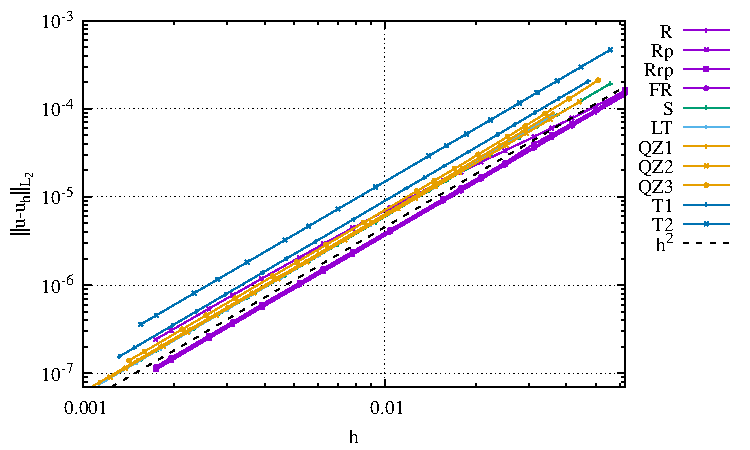
\includegraphics[width=5cm]{python_codes/fieldstone_78/results/errors_u_exp1.pdf}
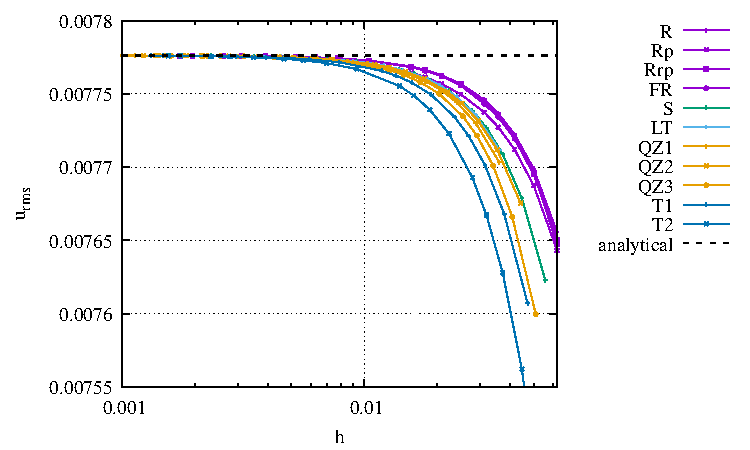
\includegraphics[width=5cm]{python_codes/fieldstone_78/results/vrms_exp1.pdf} 
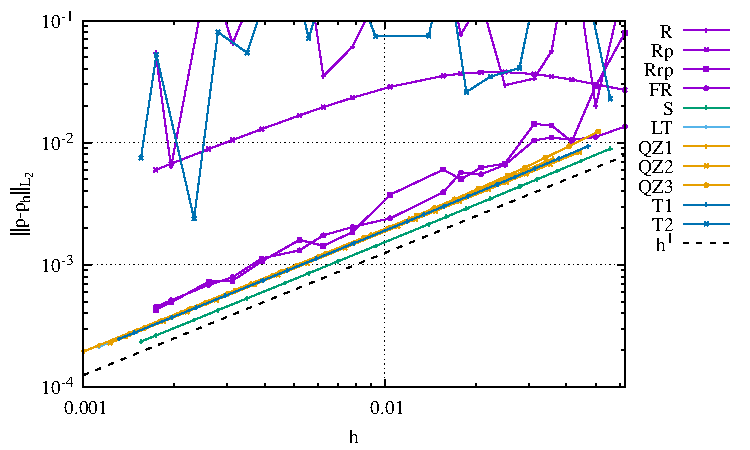
\includegraphics[width=5cm]{python_codes/fieldstone_78/results/errors_p_exp1.pdf}\\
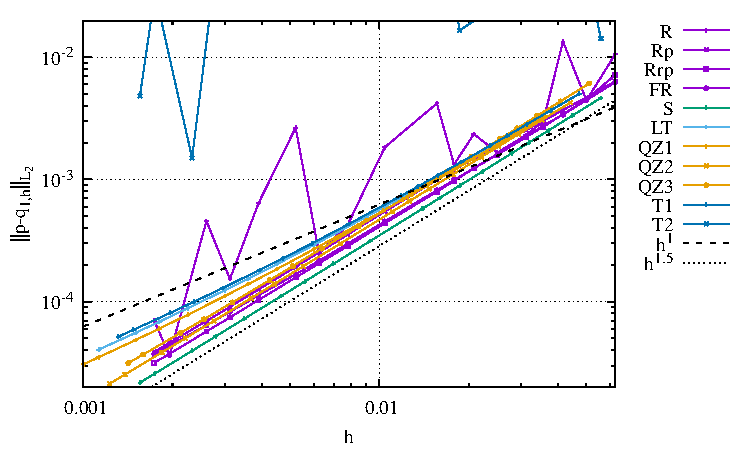
\includegraphics[width=5cm]{python_codes/fieldstone_78/results/errors_q1_exp1.pdf}
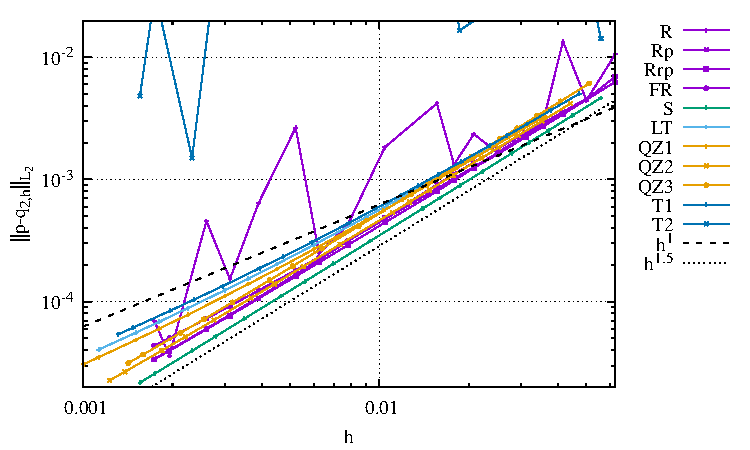
\includegraphics[width=5cm]{python_codes/fieldstone_78/results/errors_q2_exp1.pdf}
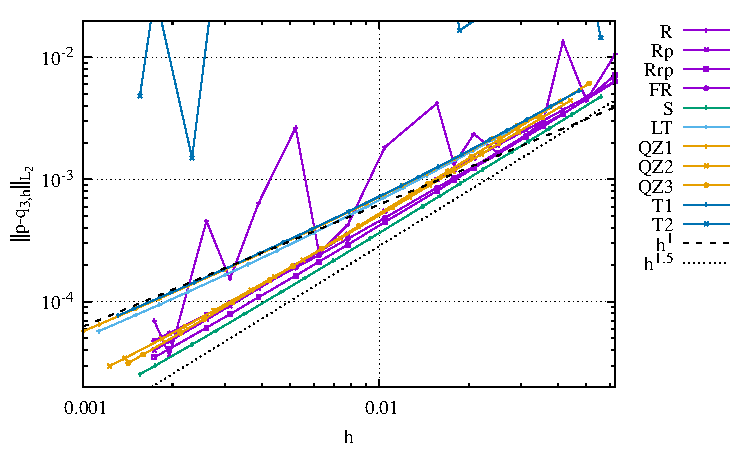
\includegraphics[width=5cm]{python_codes/fieldstone_78/results/errors_q3_exp1.pdf}\\
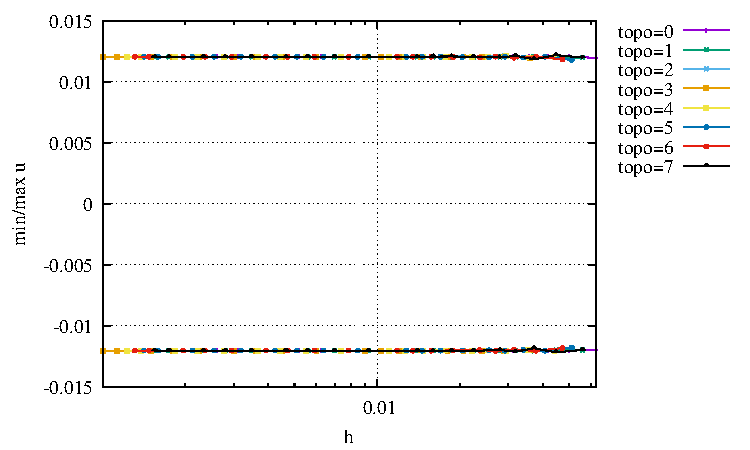
\includegraphics[width=5cm]{python_codes/fieldstone_78/results/stats_u_exp1.pdf}
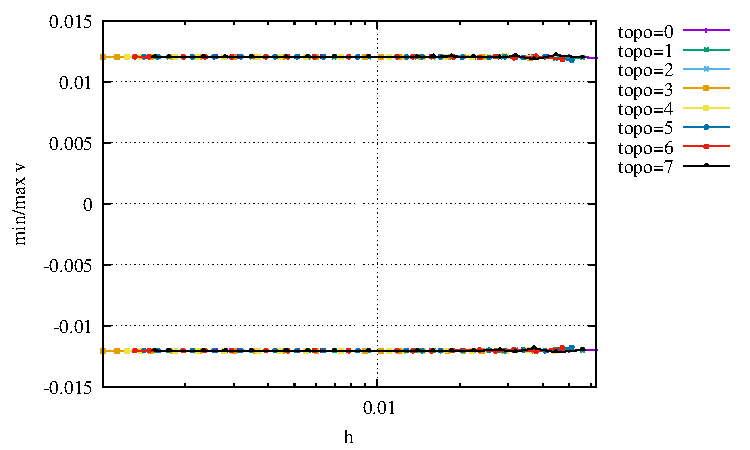
\includegraphics[width=5cm]{python_codes/fieldstone_78/results/stats_v_exp1.pdf}\\
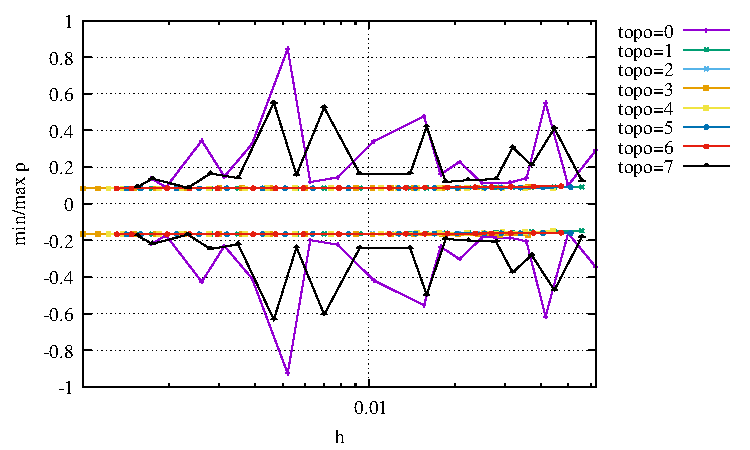
\includegraphics[width=5cm]{python_codes/fieldstone_78/results/stats_p_exp1.pdf}\\
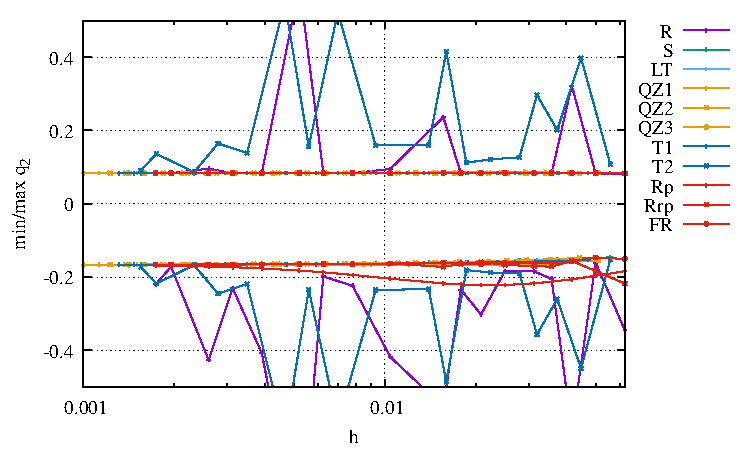
\includegraphics[width=5cm]{python_codes/fieldstone_78/results/stats_q1_exp1.pdf}
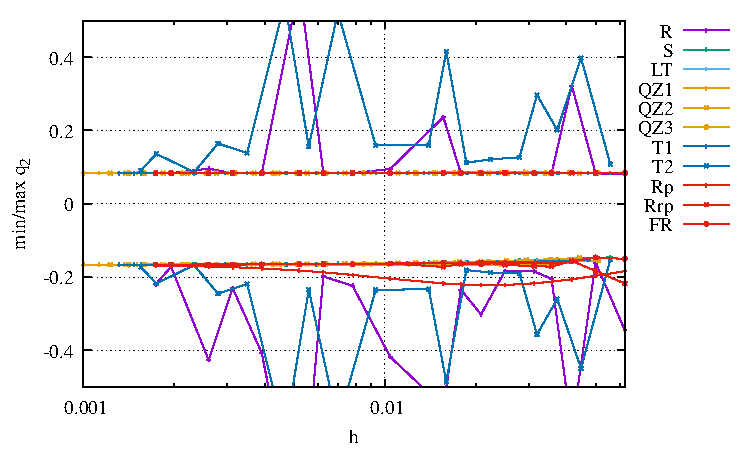
\includegraphics[width=5cm]{python_codes/fieldstone_78/results/stats_q2_exp1.pdf}
\end{center}

On the following figures the pressure is plotted against the analytical solution and 
we see that there is no checkerboarding occurring:
Rather interestingly the pressure error is the largest next to the boundaries.

\begin{center}
0)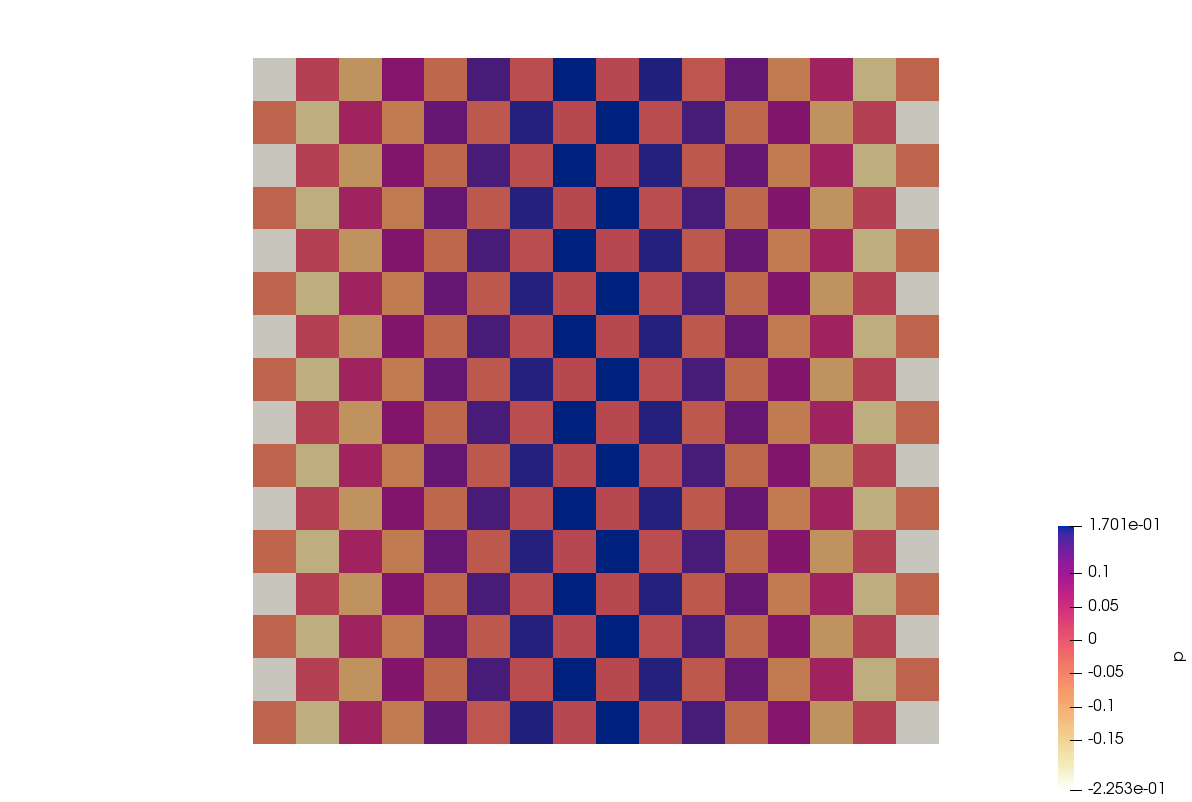
\includegraphics[width=4cm]{python_codes/fieldstone_78/results/exp01/16x16/p0}
1)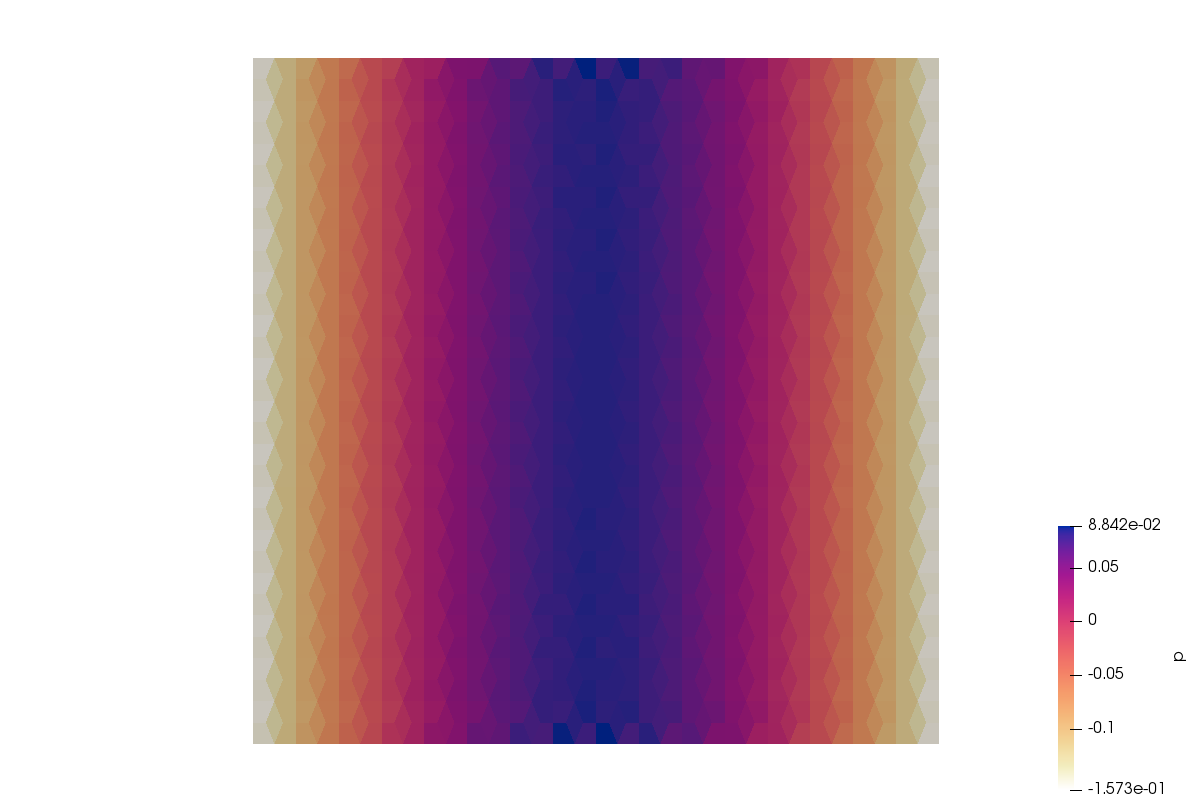
\includegraphics[width=4cm]{python_codes/fieldstone_78/results/exp01/16x16/p1}
2)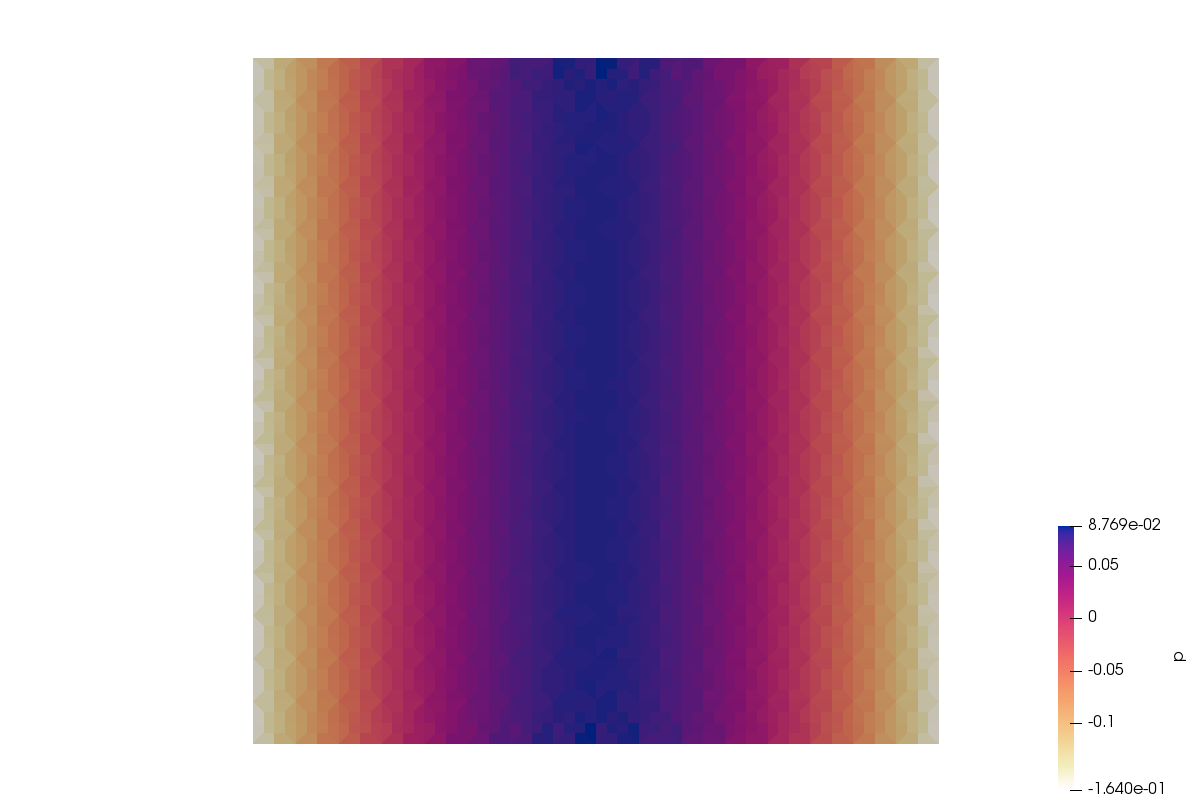
\includegraphics[width=4cm]{python_codes/fieldstone_78/results/exp01/16x16/p2}
3)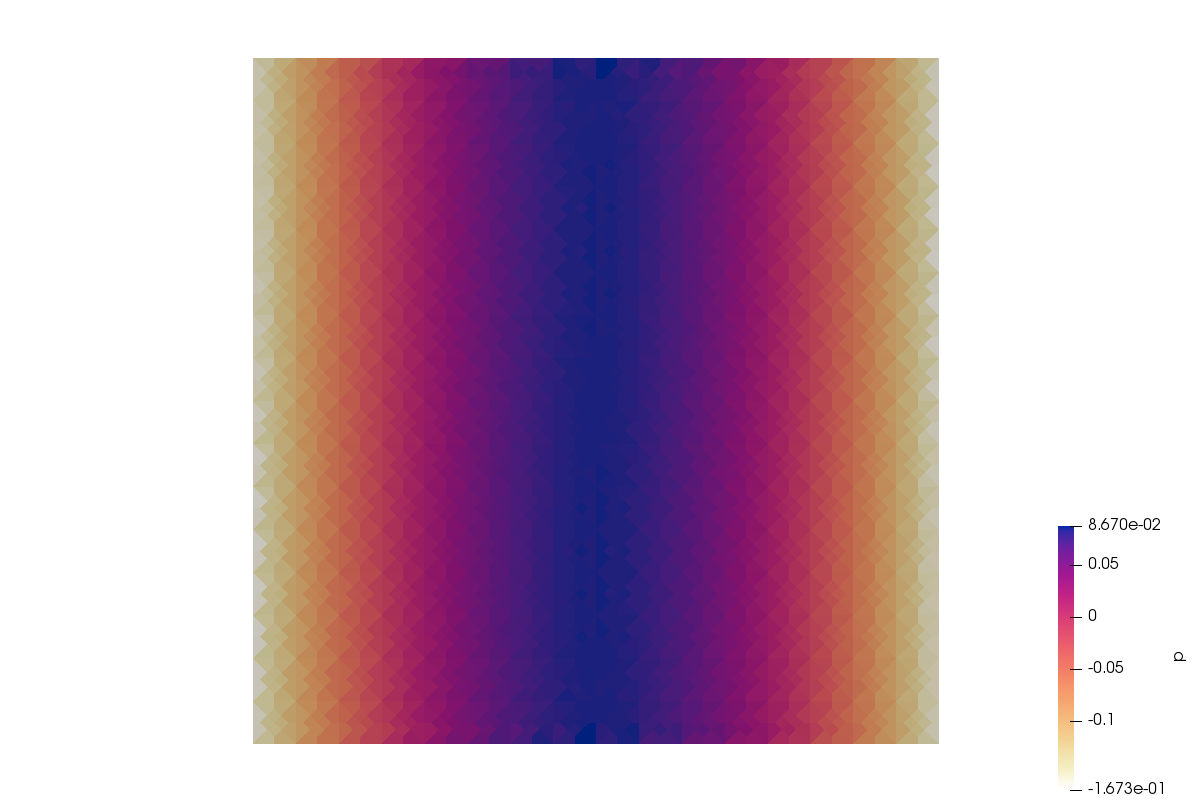
\includegraphics[width=4cm]{python_codes/fieldstone_78/results/exp01/16x16/p3}\\
4)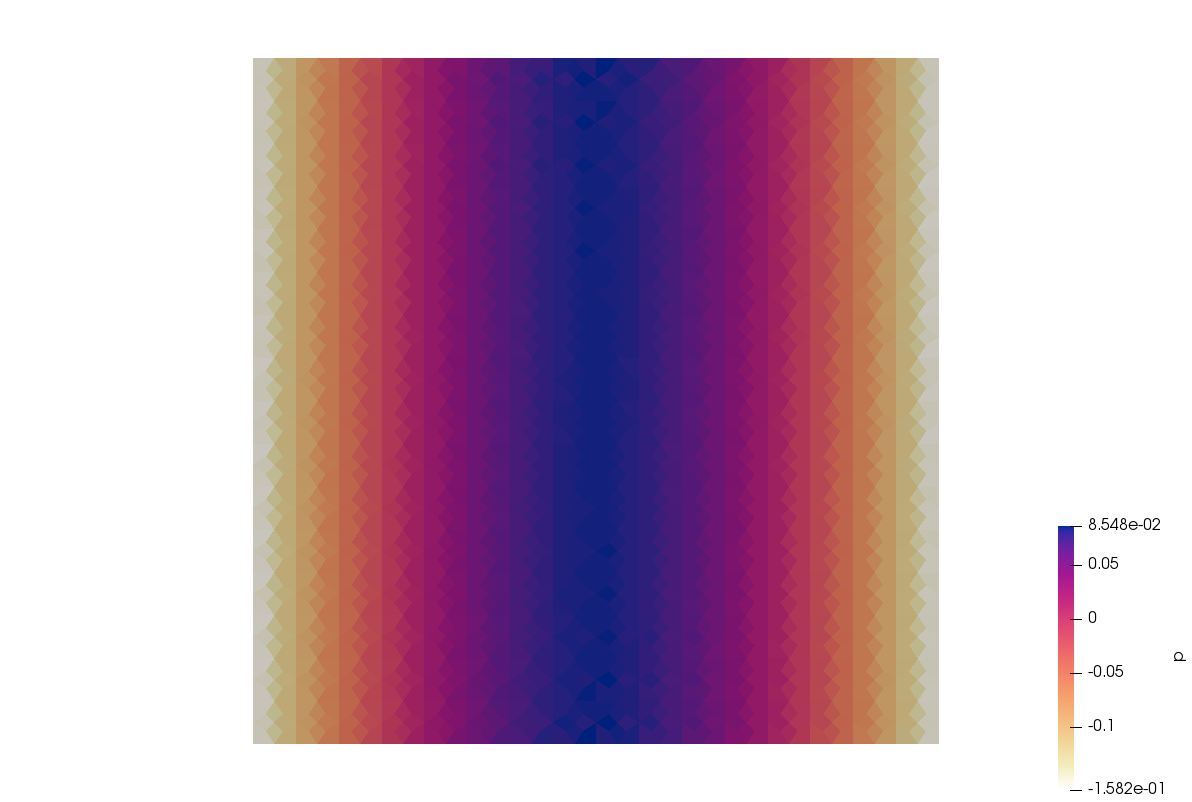
\includegraphics[width=4cm]{python_codes/fieldstone_78/results/exp01/16x16/p4}
5)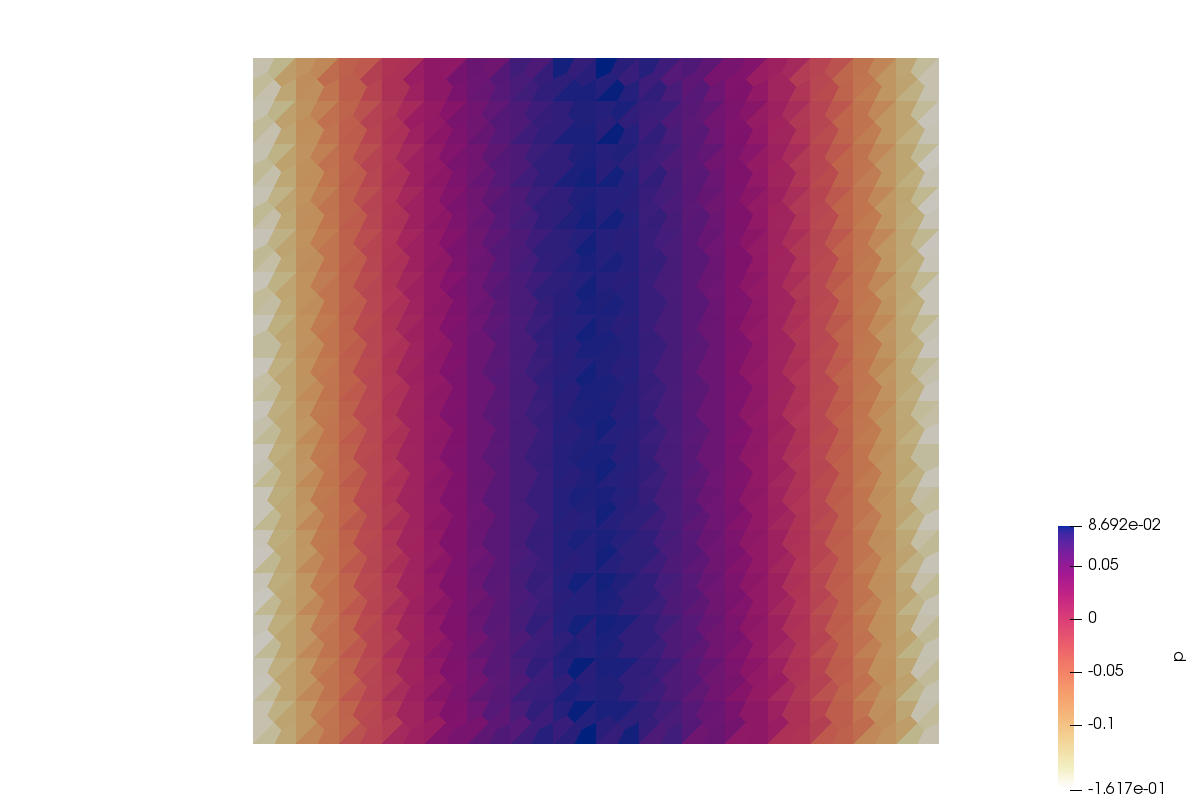
\includegraphics[width=4cm]{python_codes/fieldstone_78/results/exp01/16x16/p5}
6)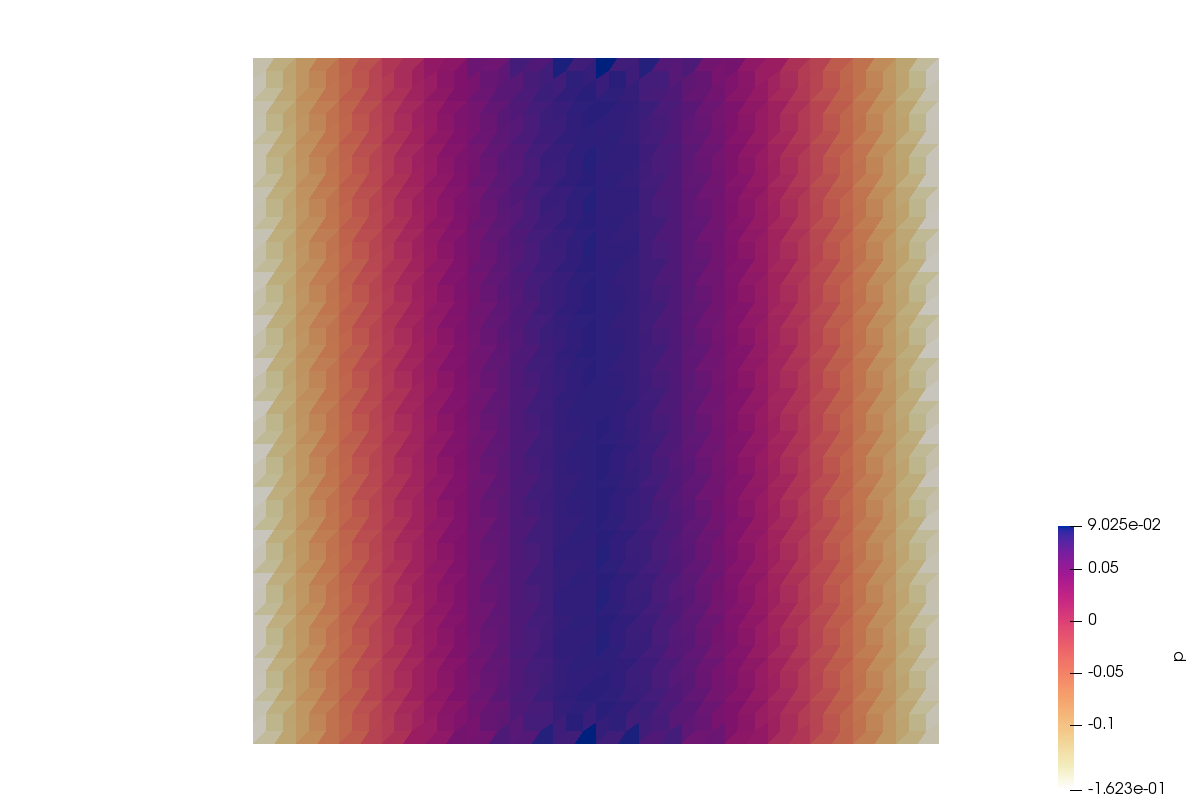
\includegraphics[width=4cm]{python_codes/fieldstone_78/results/exp01/16x16/p6}
7)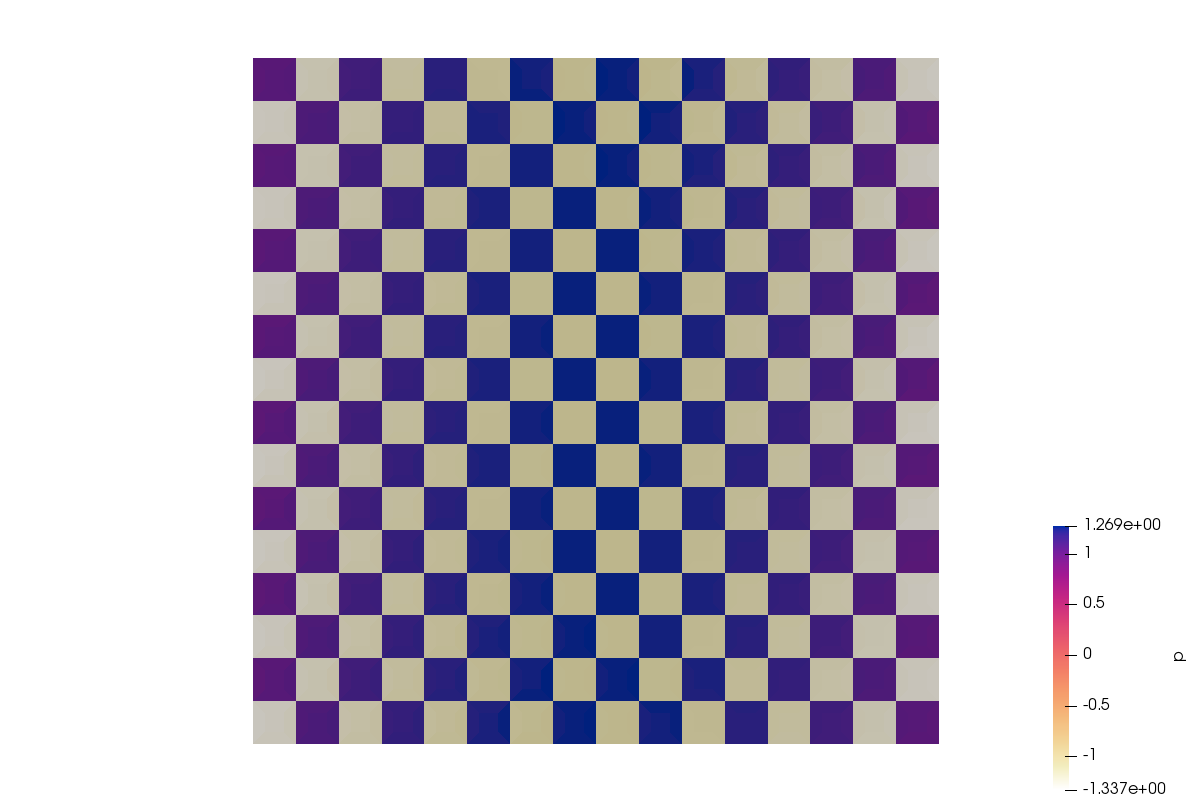
\includegraphics[width=4cm]{python_codes/fieldstone_78/results/exp01/16x16/p7}\\
{\captionfont Meshes  made of 16x16 (macro-)elements.} 
\end{center}


\newpage
%-------------------------------------------------------------
\subsection*{Experiment 2: Dimensionless sinking square (EXP)}

The block has size $0.25\times 0.25$, centered in the domain. No-slip boundary conditions are imposed on all 
sides. The buoyancy force $\rho g_y$ is -1 in the block and zero elsewhere. Viscosity is constant and 
equal to 1 everywhere. 

\begin{center}
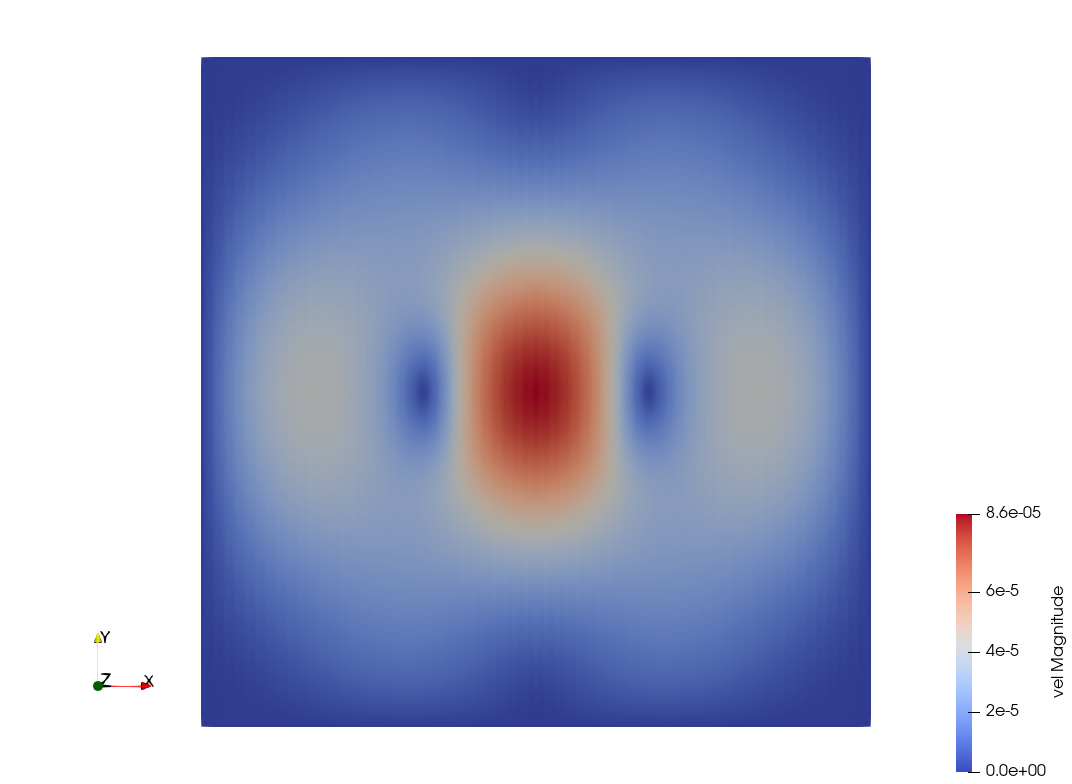
\includegraphics[width=5cm]{python_codes/fieldstone_78/results/exp02/vel}
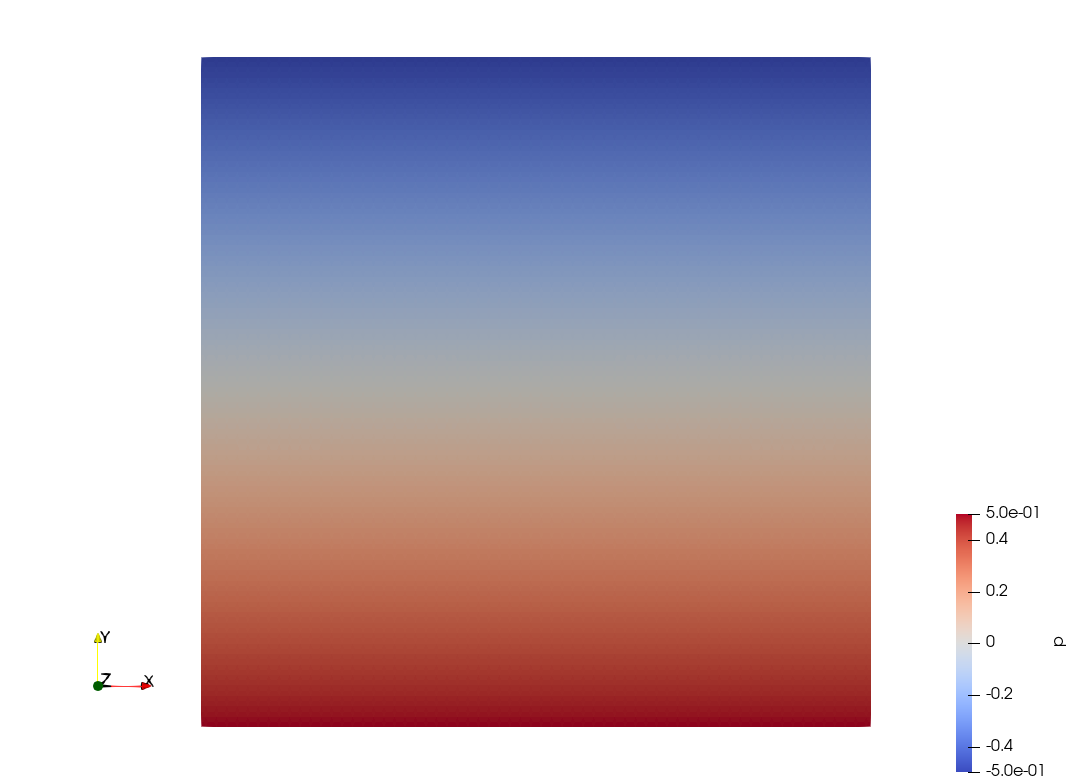
\includegraphics[width=5cm]{python_codes/fieldstone_78/results/exp02/p}
\includegraphics[width=5cm]{python_codes/fieldstone_78/results/exp02/by}\\
{\captionfont Stenberg, 64x64.}
\end{center}

\begin{center}
\includegraphics[width=5cm]{python_codes/fieldstone_78/results/vrms_exp2.pdf} 
\includegraphics[width=5cm]{python_codes/fieldstone_78/results/stats_u_exp2.pdf}
\includegraphics[width=5cm]{python_codes/fieldstone_78/results/stats_v_exp2.pdf}\\
\includegraphics[width=5cm]{python_codes/fieldstone_78/results/stats_p_exp2.pdf}
\includegraphics[width=5cm]{python_codes/fieldstone_78/results/stats_q1_exp2.pdf}
\includegraphics[width=5cm]{python_codes/fieldstone_78/results/stats_q2_exp2.pdf}
\end{center}


\begin{center}
\includegraphics[width=5cm]{python_codes/fieldstone_78/results/pressure_top_exp2.pdf}
\includegraphics[width=5cm]{python_codes/fieldstone_78/results/vx_profile_exp2.pdf}
\includegraphics[width=5cm]{python_codes/fieldstone_78/results/vy_profile_exp2.pdf}\\
{\captionfont Left: Pressure at the surface; Middle, Right: velocity on vertical line in the middle.}
\end{center}




\newpage
%-------------------------------------------------------------
\subsection*{Experiment 3: Dimensionless sinking sphere (EXP)}

This is the same experiment as above, except for the geometry of the object 
which is now a sphere of radius 0.125 so that the interface between both fluids 
is never aligned with the mesh/element edges. The sphere has density is 1 while the surrounding is 0.
Its viscosity is $10^4$ while the surrounding is 1.

\begin{center}
\includegraphics[width=4cm]{python_codes/fieldstone_78/results/exp03/vel}
\includegraphics[width=4cm]{python_codes/fieldstone_78/results/exp03/p}
\includegraphics[width=4cm]{python_codes/fieldstone_78/results/exp03/by}
\includegraphics[width=4cm]{python_codes/fieldstone_78/results/exp03/viscosity}\\
{\captionfont Stenberg, 64x64.}
\end{center}

\begin{center}
\includegraphics[width=5cm]{python_codes/fieldstone_78/results/vrms_exp3.pdf} 
\includegraphics[width=5cm]{python_codes/fieldstone_78/results/stats_u_exp3.pdf}
\includegraphics[width=5cm]{python_codes/fieldstone_78/results/stats_v_exp3.pdf}\\
\includegraphics[width=5cm]{python_codes/fieldstone_78/results/stats_p_exp3.pdf}
\includegraphics[width=5cm]{python_codes/fieldstone_78/results/stats_q1_exp3.pdf}
\includegraphics[width=5cm]{python_codes/fieldstone_78/results/stats_q2_exp3.pdf}
\end{center}

\begin{center}
\includegraphics[width=5cm]{python_codes/fieldstone_78/results/pressure_top_exp3.pdf}
\includegraphics[width=5cm]{python_codes/fieldstone_78/results/vx_profile_exp3.pdf}
\includegraphics[width=5cm]{python_codes/fieldstone_78/results/vy_profile_exp3.pdf}\\
{\captionfont Left: Pressure at the surface; Middle, Right: velocity on vertical line in the middle.}
\end{center}





\newpage
%-------------------------------------------------------------
\subsection*{Experiment 4: The aquarium (EXP)}

{\color{red} description}
Technically a manufactured solution, with $\vec{\upnu}=0$ and $p=\rho g (L_y-y)$.

\begin{center}
\includegraphics[width=5cm]{python_codes/fieldstone_78/results/vrms_exp4.pdf} 
\includegraphics[width=5cm]{python_codes/fieldstone_78/results/stats_u_exp4.pdf}
\includegraphics[width=5cm]{python_codes/fieldstone_78/results/stats_v_exp4.pdf}\\
\includegraphics[width=5cm]{python_codes/fieldstone_78/results/stats_p_exp4.pdf}
\includegraphics[width=5cm]{python_codes/fieldstone_78/results/stats_q1_exp4.pdf}
\includegraphics[width=5cm]{python_codes/fieldstone_78/results/stats_q2_exp4.pdf}
\end{center}

We see that the Stenberg macro-element is the best, with the lowest velocity and pressure errors.

\begin{center}
\includegraphics[width=5cm]{python_codes/fieldstone_78/results/pressure_top_exp4.pdf}
\includegraphics[width=5cm]{python_codes/fieldstone_78/results/vx_profile_exp4.pdf}
\includegraphics[width=5cm]{python_codes/fieldstone_78/results/vy_profile_exp4.pdf}\\
{\captionfont Left: Pressure at the surface; Middle, Right: velocity on vertical line in the middle.}
\end{center}





\newpage
%-------------------------------------------------------------
\subsection*{Experiment 5: SolKz (MS)}

{\color{red} description}

\begin{center}
\includegraphics[width=4cm]{python_codes/fieldstone_78/results/exp05/vel}
\includegraphics[width=4cm]{python_codes/fieldstone_78/results/exp05/p}
\includegraphics[width=4cm]{python_codes/fieldstone_78/results/exp05/by}
\includegraphics[width=4cm]{python_codes/fieldstone_78/results/exp05/eta}\\
{\captionfont Stenberg, 64x64.}
\end{center}


\begin{center}
\includegraphics[width=5cm]{python_codes/fieldstone_78/results/errors_u_exp5.pdf}
\includegraphics[width=5cm]{python_codes/fieldstone_78/results/vrms_exp5.pdf} \\
\includegraphics[width=5cm]{python_codes/fieldstone_78/results/errors_p_exp5.pdf}
\includegraphics[width=5cm]{python_codes/fieldstone_78/results/errors_q1_exp5.pdf}
\includegraphics[width=5cm]{python_codes/fieldstone_78/results/errors_q2_exp5.pdf}\\
\includegraphics[width=5cm]{python_codes/fieldstone_78/results/stats_u_exp5.pdf}
\includegraphics[width=5cm]{python_codes/fieldstone_78/results/stats_v_exp5.pdf}\\
\includegraphics[width=5cm]{python_codes/fieldstone_78/results/stats_p_exp5.pdf}
\includegraphics[width=5cm]{python_codes/fieldstone_78/results/stats_q1_exp5.pdf}
\includegraphics[width=5cm]{python_codes/fieldstone_78/results/stats_q2_exp5.pdf}
\end{center}

\begin{center}
\includegraphics[width=5cm]{python_codes/fieldstone_78/results/pressure_top_exp5.pdf}
\includegraphics[width=5cm]{python_codes/fieldstone_78/results/vx_profile_exp5.pdf}
\includegraphics[width=5cm]{python_codes/fieldstone_78/results/vy_profile_exp5.pdf}\\
{\captionfont Left: Pressure at the surface; Middle, Right: velocity on vertical line in the middle.}
\end{center}

plot analytical pressure and velocity against these!!




\newpage
%-------------------------------------------------------------
\subsection*{Experiment 6: Regularised Lid driven cavity (EXP)}

{\color{red} description}
Domain is 1x1. Viscosity is 1 and density is zero. 
No-slip prescribed at sides and bottom and $\vec{\upnu}=(16x^2(1-x^2),0)$ prescribed on the top.

\begin{center}
\includegraphics[width=5cm]{python_codes/fieldstone_78/results/exp06/vel}
\includegraphics[width=5cm]{python_codes/fieldstone_78/results/exp06/p}\\
{\captionfont Stenberg, 64x64.}
\end{center}

\begin{center}
\includegraphics[width=5cm]{python_codes/fieldstone_78/results/vrms_exp6.pdf} 
\includegraphics[width=5cm]{python_codes/fieldstone_78/results/stats_u_exp6.pdf}
\includegraphics[width=5cm]{python_codes/fieldstone_78/results/stats_v_exp6.pdf}\\
\includegraphics[width=5cm]{python_codes/fieldstone_78/results/stats_p_exp6.pdf}
%\includegraphics[width=5cm]{python_codes/fieldstone_78/results/stats_q1_exp6.pdf}
%\includegraphics[width=5cm]{python_codes/fieldstone_78/results/stats_q2_exp6.pdf}
\end{center}

pressure of topo 0 is 10**12 , no in plot

\begin{center}
\includegraphics[width=5cm]{python_codes/fieldstone_78/results/pressure_top_exp6.pdf}
\includegraphics[width=5cm]{python_codes/fieldstone_78/results/vx_profile_exp6.pdf}
\includegraphics[width=5cm]{python_codes/fieldstone_78/results/vy_profile_exp6.pdf}\\
{\captionfont Left: Pressure at the surface; Middle, Right: velocity on vertical line in the middle.}
\end{center}








\newpage
%-------------------------------------------------------------
\subsection*{Experiment 7: cavity (MS)}

{\color{red} description}

$eta=1$, 
\[
b_x=0 \qquad b_y=-(8x-2)
\]
\[
u=(2y-1)x(1-x)
\qquad
v=-(2x-1)y(1-y)
\qquad
p=2x(1-2y)
\]
Analytical solution is prescribed on all four sides.

\begin{center}
\includegraphics[width=5cm]{python_codes/fieldstone_78/results/errors_u_exp7.pdf}
\includegraphics[width=5cm]{python_codes/fieldstone_78/results/vrms_exp7.pdf} \\
\includegraphics[width=5cm]{python_codes/fieldstone_78/results/errors_p_exp7.pdf}
\includegraphics[width=5cm]{python_codes/fieldstone_78/results/errors_q1_exp7.pdf}
\includegraphics[width=5cm]{python_codes/fieldstone_78/results/errors_q2_exp7.pdf}\\
\includegraphics[width=5cm]{python_codes/fieldstone_78/results/stats_u_exp7.pdf}
\includegraphics[width=5cm]{python_codes/fieldstone_78/results/stats_v_exp7.pdf}\\
\includegraphics[width=5cm]{python_codes/fieldstone_78/results/stats_p_exp7.pdf}
\includegraphics[width=5cm]{python_codes/fieldstone_78/results/stats_q1_exp7.pdf}
\includegraphics[width=5cm]{python_codes/fieldstone_78/results/stats_q2_exp7.pdf}
\end{center}

\begin{center}
\includegraphics[width=5cm]{python_codes/fieldstone_78/results/pressure_top_exp7.pdf}
\includegraphics[width=5cm]{python_codes/fieldstone_78/results/vx_profile_exp7.pdf}
\includegraphics[width=5cm]{python_codes/fieldstone_78/results/vy_profile_exp7.pdf}\\
{\captionfont Left: Pressure at the surface; Middle, Right: velocity on vertical line in the middle.}
\end{center}




\newpage
%-------------------------------------------------------------
\subsection*{Experiment 8: Earth-sized sinking block (EXP)}

Earth dimensions. 

\begin{center}
\includegraphics[width=5cm]{python_codes/fieldstone_78/results/exp08/vel}
\includegraphics[width=5cm]{python_codes/fieldstone_78/results/exp08/p}
\includegraphics[width=5cm]{python_codes/fieldstone_78/results/exp08/eta}\\
{\captionfont Stenberg, 64x64.}
\end{center}


\begin{center}
\includegraphics[width=5cm]{python_codes/fieldstone_78/results/exp08/p_block_res32.pdf}
\includegraphics[width=5cm]{python_codes/fieldstone_78/results/exp08/p_block_res64.pdf}\\
\includegraphics[width=5cm]{python_codes/fieldstone_78/results/exp08/q1_block_res32.pdf}
\includegraphics[width=5cm]{python_codes/fieldstone_78/results/exp08/q1_block_res64.pdf}\\
\includegraphics[width=5cm]{python_codes/fieldstone_78/results/exp08/v_block_res32.pdf}
\includegraphics[width=5cm]{python_codes/fieldstone_78/results/exp08/v_block_res64.pdf}\\
%\includegraphics[width=5cm]{python_codes/fieldstone_78/results/exp08/pressure_top_res32.pdf}
%\includegraphics[width=5cm]{python_codes/fieldstone_78/results/exp08/pressure_top_res64.pdf}\\
%\includegraphics[width=5cm]{python_codes/fieldstone_78/results/exp08/v_profile_res32.pdf}
%\includegraphics[width=5cm]{python_codes/fieldstone_78/results/exp08/v_profile_res64.pdf}
\end{center}


\newpage
\begin{center}
\includegraphics[width=4cm]{python_codes/fieldstone_78/results/exp08/vel_profile_topo0_full.pdf}
\includegraphics[width=4cm]{python_codes/fieldstone_78/results/exp08/vel_profile_topo1_full.pdf}
\includegraphics[width=4cm]{python_codes/fieldstone_78/results/exp08/vel_profile_topo2_full.pdf}
\includegraphics[width=4cm]{python_codes/fieldstone_78/results/exp08/vel_profile_topo3_full.pdf}\\
\includegraphics[width=4cm]{python_codes/fieldstone_78/results/exp08/vel_profile_topo4_full.pdf}
\includegraphics[width=4cm]{python_codes/fieldstone_78/results/exp08/vel_profile_topo5_full.pdf}
\includegraphics[width=4cm]{python_codes/fieldstone_78/results/exp08/vel_profile_topo6_full.pdf}
\includegraphics[width=4cm]{python_codes/fieldstone_78/results/exp08/vel_profile_topo7_full.pdf}
\end{center}


\begin{center}
\includegraphics[width=4cm]{python_codes/fieldstone_78/results/exp08/vel_profile_topo0_reduced.pdf}
\includegraphics[width=4cm]{python_codes/fieldstone_78/results/exp08/vel_profile_topo1_reduced.pdf}
\includegraphics[width=4cm]{python_codes/fieldstone_78/results/exp08/vel_profile_topo2_reduced.pdf}
\includegraphics[width=4cm]{python_codes/fieldstone_78/results/exp08/vel_profile_topo3_reduced.pdf}\\
\includegraphics[width=4cm]{python_codes/fieldstone_78/results/exp08/vel_profile_topo4_reduced.pdf}
\includegraphics[width=4cm]{python_codes/fieldstone_78/results/exp08/vel_profile_topo5_reduced.pdf}
\includegraphics[width=4cm]{python_codes/fieldstone_78/results/exp08/vel_profile_topo6_reduced.pdf}
\includegraphics[width=4cm]{python_codes/fieldstone_78/results/exp08/vel_profile_topo7_reduced.pdf}
\end{center}











\newpage
%-------------------------------------------------------------
\subsection*{Experiment 9: Dohrmann \& Bochev (MS)}

It is described in Section~\ref{MMS-mms_dobo}. 
This benchmark is also used in Worthen \etal \cite{wosp14} and Lamichhane \etal \cite{lami17}.
It is for a unit square with $\nu=\eta/\rho=1$ and the smooth exact solution is
\begin{eqnarray}
u(x,y) &=& x+x^2 - 2xy+x^3 - 3xy^2 + x^2y \\
v(x,y) &=& -y-2xy+y^2 -3x^2y + y^3 - xy^2 \\
p(x,y) &=& xy+x+y+x^3y^2 - 4/3
\end{eqnarray}
Note that the pressure field is such that $\int_{\Omega} p \; dV = 0$.

\begin{center}
\includegraphics[width=5cm]{python_codes/fieldstone_78/results/errors_u_exp9.pdf}
\includegraphics[width=5cm]{python_codes/fieldstone_78/results/vrms_exp9.pdf} \\
\includegraphics[width=5cm]{python_codes/fieldstone_78/results/errors_p_exp9.pdf}
\includegraphics[width=5cm]{python_codes/fieldstone_78/results/errors_q1_exp9.pdf}
\includegraphics[width=5cm]{python_codes/fieldstone_78/results/errors_q2_exp9.pdf}\\
\includegraphics[width=5cm]{python_codes/fieldstone_78/results/stats_u_exp9.pdf}
\includegraphics[width=5cm]{python_codes/fieldstone_78/results/stats_v_exp9.pdf}\\
\includegraphics[width=5cm]{python_codes/fieldstone_78/results/stats_p_exp9.pdf}
\includegraphics[width=5cm]{python_codes/fieldstone_78/results/stats_q1_exp9.pdf}
\includegraphics[width=5cm]{python_codes/fieldstone_78/results/stats_q2_exp9.pdf}
\end{center}





\newpage
%-------------------------------------------------------------
\subsection*{Experiment 10: flow around square cylinder (EXP)}

This experiment is inspired by the very common one found in CFD: a laminar flow 
is forced to go around a cylinder (circular or square cross section) often 
generating turbulence in its wake for high-enough Reynolds number Navier-Stokes flow.

The domain is 4x1. Free slip boundary conditions are imposed top and bottom. 
A horizontal flow $\vec{v}=(0,1)$ is prescribed on the left boundary, and the 
right boundary is left open. All the nodes on a square centered in the middle of the domain 
of size 0.125x0.125 are set to no-slip boundary conditions.
Viscosity is one and gravity is switched off.

\begin{center}
\includegraphics[width=5cm]{python_codes/fieldstone_78/results/exp10/vel}
\includegraphics[width=5cm]{python_codes/fieldstone_78/results/exp10/p}
\end{center}

\begin{center}
\includegraphics[width=5cm]{python_codes/fieldstone_78/results/vrms_exp10.pdf} 
\includegraphics[width=5cm]{python_codes/fieldstone_78/results/stats_u_exp10.pdf}
\includegraphics[width=5cm]{python_codes/fieldstone_78/results/stats_v_exp10.pdf}\\
\includegraphics[width=5cm]{python_codes/fieldstone_78/results/stats_p_exp10.pdf}
\includegraphics[width=5cm]{python_codes/fieldstone_78/results/stats_q1_exp10.pdf}
\includegraphics[width=5cm]{python_codes/fieldstone_78/results/stats_q2_exp10.pdf}
\end{center}




\newpage
%-------------------------------------------------------------
\subsection*{Experiment 11: flow over cavity (EXP)}

The domain is 4x1. No slip boundary conditions are imposed on all walls.
The cavity is formed by prescribing $\vec{\upnu}=\vec{0}$ on the desired 
nodes inside the domain. $\vec{\upnu}(x,y)=-(y-L_y)(y-L_y/2)$ is prescribed 
on the left inflow boundary while $\upnu_y=0$ is prescribed on the outflow boundary.
Viscosity is one and gravity is switched off.
 
\begin{center}
\includegraphics[width=5cm]{python_codes/fieldstone_78/results/exp11/vel}
\includegraphics[width=5cm]{python_codes/fieldstone_78/results/exp11/p}
\end{center}

\begin{center}
\includegraphics[width=5cm]{python_codes/fieldstone_78/results/vrms_exp11.pdf} 
\includegraphics[width=5cm]{python_codes/fieldstone_78/results/stats_u_exp11.pdf}
\includegraphics[width=5cm]{python_codes/fieldstone_78/results/stats_v_exp11.pdf}\\
\includegraphics[width=5cm]{python_codes/fieldstone_78/results/stats_p_exp11.pdf}
\includegraphics[width=5cm]{python_codes/fieldstone_78/results/stats_q1_exp11.pdf}
\includegraphics[width=5cm]{python_codes/fieldstone_78/results/stats_q2_exp11.pdf}
\end{center}







\newpage
%-------------------------------------------------------------
\subsection*{Experiment 12: flow over obstacle (EXP)}

Domain is 4x1. Viscosity is 1, $\rho g = -1$. Free slip top and bottom.
Obstacle consists of nodes ($x=L_x/2$ and $y\le L_y/2$) where $\vec\upnu=0$. 
$\vec\upnu=(1,0)$ prescribed on the left, $\upnu_y=0$ on the right.

\begin{center}
\includegraphics[width=5cm]{python_codes/fieldstone_78/results/exp12/vel}
\includegraphics[width=5cm]{python_codes/fieldstone_78/results/exp12/p}
\end{center}

\begin{center}
\includegraphics[width=5cm]{python_codes/fieldstone_78/results/vrms_exp12.pdf} 
\includegraphics[width=5cm]{python_codes/fieldstone_78/results/stats_u_exp12.pdf}
\includegraphics[width=5cm]{python_codes/fieldstone_78/results/stats_v_exp12.pdf}\\
\includegraphics[width=5cm]{python_codes/fieldstone_78/results/stats_p_exp12.pdf}
\includegraphics[width=5cm]{python_codes/fieldstone_78/results/stats_q1_exp12.pdf}
\includegraphics[width=5cm]{python_codes/fieldstone_78/results/stats_q2_exp12.pdf}
\end{center}







\newpage
%-------------------------------------------------------------
\subsection*{Experiment 13: SolCx (MS)}

\begin{figure}
\centering
\includegraphics[width=5cm]{python_codes/fieldstone_78/images/fields/vel_solcx}
\includegraphics[width=5cm]{python_codes/fieldstone_78/images/fields/press_solcx}\\
{\captionfont Velocity and pressure fields for SolCx experiment.}
\end{figure}

For SolKz the viscosity is given by $\eta(y)=\exp(By)$ with $B=\ln 10^6 \simeq 13.8155$ 
and the density field by $\rho(x,y)=\sin(2y) \cos(3\pi x)$, with 


\begin{figure}
\centering
\includegraphics[width=5cm]{python_codes/fieldstone_78/results/errors_u_exp13}
\includegraphics[width=5cm]{python_codes/fieldstone_78/results/vrms_exp13} \\
\includegraphics[width=5cm]{python_codes/fieldstone_78/results/errors_p_exp13}
\includegraphics[width=5cm]{python_codes/fieldstone_78/results/errors_q1_exp13}
{\captionfont SolCx benchmark: velocity error, 
root mean square velocity, elemental pressure error and nodal pressure error
as a function of the the average mesh size $h$.} 
\end{figure}



Remark: Le Tallec macro-element has vertical line in the middle, so that 
even/odd does not matter, there is always an element edge aligned with x=1/2.



\newpage
%-------------------------------------------------------------
\subsection*{Experiment 14: solvi (MS)}

\begin{center}
\includegraphics[width=5cm]{python_codes/fieldstone_78/results/exp14/vel}
\includegraphics[width=5cm]{python_codes/fieldstone_78/results/exp14/p}
\end{center}


\begin{center}
\includegraphics[width=5cm]{python_codes/fieldstone_78/results/errors_u_exp14.pdf}
\includegraphics[width=5cm]{python_codes/fieldstone_78/results/vrms_exp14.pdf} \\
\includegraphics[width=5cm]{python_codes/fieldstone_78/results/errors_p_exp14.pdf}
\includegraphics[width=5cm]{python_codes/fieldstone_78/results/errors_q1_exp14.pdf}
\includegraphics[width=5cm]{python_codes/fieldstone_78/results/errors_q2_exp14.pdf}\\
\includegraphics[width=5cm]{python_codes/fieldstone_78/results/stats_u_exp14.pdf}
\includegraphics[width=5cm]{python_codes/fieldstone_78/results/stats_v_exp14.pdf}\\
\includegraphics[width=5cm]{python_codes/fieldstone_78/results/stats_p_exp14.pdf}
\includegraphics[width=5cm]{python_codes/fieldstone_78/results/stats_q1_exp14.pdf}
\includegraphics[width=5cm]{python_codes/fieldstone_78/results/stats_q2_exp14.pdf}
\end{center}







\newpage
%%%%%%%%%%%%%%%%%%%%%%%%%%%%%%%%%%%%%%%%%%%%%%%%%%%%%%%%%%%%%%%%%%%%%%%%%%%%%%%%%%%%%%%%%%%%

\section*{Discussion}

Intro starts from conclusion of thba22 about Q1P0

3D?

annulus?

use schur complement solver to show it is stable ?

cmat version ? 


is $<h>$ best? smthg fancier ?

remark in Gang Lu paper with Dave, about removing checkerboard mode

I have the feeling results can be different if i impose the
constraint in the matrix like it was at first?

what is the real advantage of such a macro-element? it is LBB stable, so 
iterative solver will work optimally, and the pressure has no checkerboard.
Also the number of non-zeros per line of the matrix is small.  
On the other hand it is anisotropic since the 'diamonds are vertical'. 
Also if one would consider a macro-element as an element, it counts 10 velocity nodes and 5 pressures, 
which makes it much more expensive than a $Q_2\times Q_1$ element of the same size...
We find that toplogy 7 does not yield a stable macroelement, so it will be discarded in 
future tests/experiments.

various stabilisations have been proposed for q1p0. However they invariably 
rely on adding a block in the Stokes matrix \ref{XXXX} or altering the 
linear solver so as to filter the spurious modes. 
We here focus on techniques that only involve a specific mesh topology and 
no other modification.
Furthermode it is the author's experimence that 
macro-elt stabilisations are not compatible with buoyancy driven flow

check \cite{nath93}


%......................................................................
\paragraph{A note about the aspect ratio of the stenberg m-e.}
Let us assume that the Stenberg macro-element is $h$ high and $H=\lambda h$ long
as shown here:

\begin{center}
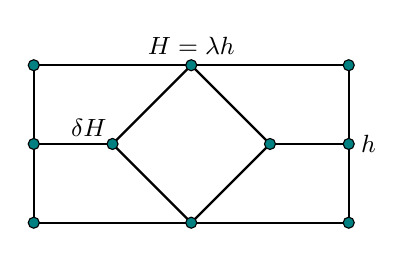
\begin{tikzpicture}
%\draw[fill=gray!23,gray!23](0,0) rectangle (5,5);
%\draw[step=0.5cm,gray,very thin] (0,0) grid (6,4); %background grid
\draw[thick] (1,1) -- (5,1) -- (5,3) -- (1,3) -- cycle;  
\draw[thick] (3,1) -- (4,2) -- (3,3) -- (2,2) -- cycle;  
\draw[thick] (1,2) -- (2,2);  
\draw[thick] (4,2) -- (5,2);  
\node[] at (5.25,2) {\small $h$};
\node[] at (3,3.25) {\small $H=\lambda h$};
\node[] at (1.7,2.2) {\small $\delta H$};
\draw[black,fill=teal] (1,1) circle (2pt);
\draw[black,fill=teal] (3,1) circle (2pt);
\draw[black,fill=teal] (5,1) circle (2pt);
\draw[black,fill=teal] (1,2) circle (2pt);
\draw[black,fill=teal] (2,2) circle (2pt);
\draw[black,fill=teal] (4,2) circle (2pt);
\draw[black,fill=teal] (5,2) circle (2pt);
\draw[black,fill=teal] (1,3) circle (2pt);
\draw[black,fill=teal] (3,3) circle (2pt);
\draw[black,fill=teal] (5,3) circle (2pt);
\end{tikzpicture}
\end{center}

The total area is 
\[
A= \lambda h \cdot h = \lambda h^2
\]
The area of the trapezes is
\[
A_{TR} = (\frac{H}{2} + \delta H)\frac12 \cdot \frac{h}{2}=\frac{\lambda h^2}{4} \left(\frac12 + \delta \right)
\]
while the area of the middle diamond is
\[
A_D = 4 \cdot \frac12 \frac{h}{2} \left(\frac{H}{2}-\delta H \right) 
= \lambda h^2 \left(\frac12 - \delta \right)
\]
We can compute $\delta$ by requiring that the trapezes and the diamond all 
have the same area, i.e.
\[
\frac{\lambda h^2}{4} (\frac12 + \delta)
=
\lambda h^2 (\frac12 - \delta)
\qquad
\Rightarrow \quad \delta = 0.3
\]
We find that the value of $\delta$ is independent of $\lambda$.

We see in the literature \cite{sten84,brfo,chba93}  that the 
macro-element is often depicted with the diamond being a square.
In this case we must have along the horizontal middle line
\[
\lambda h = 0.3 \lambda h + \frac{h}{2}+ \frac{h}{2} + 0.3 \lambda h
\qquad
\Rightarrow \quad 
\lambda=5/2
\]
The 5:2 aspect ratio macro-element guarantees equal areas and a square middle element.

But does the aspect ratio matter in practice? 
Results are shown hereunder for the D\&H benchmark:

\begin{center}
\includegraphics[width=5.7cm]{python_codes/fieldstone_78/results/exp01/stenberg_study/errors_u.pdf}
\includegraphics[width=5.7cm]{python_codes/fieldstone_78/results/exp01/stenberg_study/errors_p.pdf}
\includegraphics[width=5.7cm]{python_codes/fieldstone_78/results/exp01/stenberg_study/errors_q1.pdf}\\
{\captionfont square ($nelx=nely$): 16x16, 32x32, 48x48; 
ar ($nely/nelx=5/2$) : 10x25, 20x50, 40x100.}
\end{center}

We find that in practice this consideration does not make much of a difference,
and that the $nelx=nely$ case actually yields slightly better results.

%......................................................................
\paragraph{A note about the Le Talle m-e.}

\begin{center}
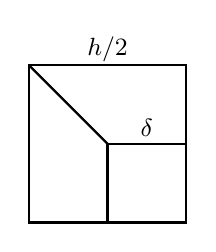
\begin{tikzpicture}
\draw[thick] (1,1) -- (3,1) -- (3,3) -- (1,3) -- cycle;  
\draw[thick] (1,3) -- (2,2);  
\draw[thick] (2,1) -- (2,2) --(3,2);  
\node[] at (2.5,2.2) {\small $\delta$};
\node[] at (2,3.2) {\small $h/2$};
\end{tikzpicture}
\end{center}

The area of the trapezes is 
\[
A_{TR}=\frac12 (\frac{h}{2}+\delta) (\frac{h}{2}-\delta) = \frac{h^2}{8}- \frac{\delta^2}{2}
\]
while the area of the square element is $A_{SQ}=\delta^2$.
When set to be equal, we arrive at
\[
\delta^2 = \frac{h}{\sqrt{12}} \simeq 0.288 h
\]


\begin{center}
\includegraphics[width=5.7cm]{python_codes/fieldstone_78/results/epsilon_studies/LT/errorss.pdf}
\end{center}





